\documentclass[xcolor=table, 8pt]{beamer}

\usetheme[progressbar=foot, sectionpage=none]{metropolis}           % Use metropolis theme

\usepackage{pifont}
\usepackage{booktabs}
\usepackage{appendixnumberbeamer}
\usepackage{colortbl}
\usepackage[font=small,labelfont=bf]{caption}
\usepackage{subcaption}
\usepackage{multirow}
\usepackage[style=authoryear, labelnumber]{biblatex}
\usepackage{xparse}
\usepackage[absolute,overlay]{textpos}
\usepackage{fontawesome5}
\usepackage{algorithm,algorithmic}
\usepackage{nameref}
\usepackage{adjustbox}
\usepackage{tikz}
\usepackage{url}
\usetikzlibrary{positioning}

\makeatletter
\newcommand*{\currentname}{\@currentlabelname}
\makeatother
\usetikzlibrary{calc,shapes.arrows,decorations.pathreplacing, decorations.text}
\addbibresource{bibliography.bib}



\setbeamerfont{caption}{size=\tiny}

\usepackage{totcount}

\newcounter{totalsection}
\regtotcounter{totalsection}

\AtBeginDocument{%
    \pretocmd{\section}{\refstepcounter{totalsection}}{\typeout{Yes, prepending was successful}}{\typeout{No, prepending was not it was successful}}%
}%

\makeatletter
\setbeamertemplate{footline}
{
  \leavevmode%
  \hbox{%
  \begin{beamercolorbox}[wd=.95\paperwidth,ht=2.25ex,dp=1ex,left]{author in head/foot}%
    % \usebeamerfont{author in head/foot} Pierre Le Jeune - 
    \hspace*{1em} \usebeamerfont{title in head/foot}\insertshorttitle\hspace*{3em}
  \end{beamercolorbox}%
  \begin{beamercolorbox}[wd=.05\paperwidth,ht=2.25ex,dp=1ex,right]{title in head/foot}%

    \insertframenumber{} \hspace*{1ex}
  \end{beamercolorbox}}%
  \vskip0pt%
  \setlength{\metropolis@progressinheadfoot@linewidth}{1pt}
  \setlength{\metropolis@titleseparator@linewidth}{1pt}
  \setlength{\metropolis@progressonsectionpage@linewidth}{1pt}
  \typeout{Section}
  \typeout{\thesection}
  \typeout{Tot section}
  \typeout{\totvalue{totalsection}}
  % \typeout{Ratio}
  % \typeout{\ratio{\thesection pt}{\totvalue{totalsection}}
  \setlength{\metropolis@progressonsectionpage}{%
    \textwidth * \ratio{\insertframenumber pt}{\inserttotalframenumber pt}%
  }%
  \begin{beamercolorbox}[wd=\paperwidth]{progress bar in head/foot}
    \begin{tikzpicture}
      \fill[bg] (0,0) rectangle (\textwidth, \metropolis@progressonsectionpage@linewidth);
      \fill[fg] (0,0) rectangle (\metropolis@progressonsectionpage, \metropolis@progressonsectionpage@linewidth);
    \end{tikzpicture}%
  \end{beamercolorbox}

}
\makeatother


% \makeatletter
% \setlength{\metropolis@progressinheadfoot@linewidth}{1pt}
% \setlength{\metropolis@titleseparator@linewidth}{1pt}
% \setlength{\metropolis@progressonsectionpage@linewidth}{1pt}

% \setbeamertemplate{progress bar in section page}{
%   \setlength{\metropolis@progressonsectionpage}{%
%     \textwidth * \ratio{\insertframenumber pt}{\inserttotalframenumber pt}%
%   }%
%   \begin{tikzpicture}
%     \fill[bg] (0,0) rectangle (\textwidth, \metropolis@progressonsectionpage@linewidth);
%     \fill[fg] (0,0) rectangle (\metropolis@progressonsectionpage, \metropolis@progressonsectionpage@linewidth);
%   \end{tikzpicture}%
% }
% \makeatother





\usepackage{tabto}    
\newcommand\sectiontab{\tab \hspace{-5.7cm}}

\newenvironment{sectionframe}[1]
  {
    \begin{frame}{\thesection. \sectiontab #1}
  }
  {
    \end{frame}
  }

  \newenvironment{subsectionframe}[1]
  {
    \begin{frame}{\thesection.\thesubsection \sectiontab #1 - \currentname}
  }
  {
    \end{frame}
  }

  \newenvironment{subsectionframemod}[1]
  {
    \begin{frame}{\thesection.\thesubsection \sectiontab \currentname}
  }
  {
    \end{frame}
  }
\newenvironment{tickenv}
  {\only{%
  \setbeamertemplate{itemize item}{\textbullet}
  \setbeamertemplate{itemize subitem}{\textbullet}
  \setbeamertemplate{itemize subsubitem}{\textbullet}}}
  {}


% Change bibliography font size
\renewcommand*{\bibfont}{\tiny}
% Change bibliography item label size
\renewcommand{\pgfuseimage}[1]{\scalebox{.75}{\includegraphics{#1}}}

% Change bibliography left margin
\defbibenvironment{bibliography}
  {\list{}
     {\settowidth{\labelwidth}{\usebeamertemplate{bibliography item}}%
      \setlength{\leftmargin}{\labelwidth}%
      \setlength{\rightmargin}{\labelwidth}%
      \setlength{\labelsep}{\biblabelsep}%
      \addtolength{\leftmargin}{\labelsep}%
      \setlength{\itemsep}{\bibitemsep}%
      \setlength{\parsep}{\bibparsep}}}
  {\endlist}
  {\item}


% \newcommand{\graphicsbox}[3]{
%   \begin{tikzpicture}
%     \node[anchor=south west,inner sep=0] (image) at (0,0) {\includegraphics[width=0.9\textwidth]{#1}};
%     \begin{scope}[x={(image.south east)},y={(image.north west)}]
%         \draw[red,ultra thick] (0.62,0.65) rectangle (0.78,0.75);
%     \end{scope}
%   \end{tikzpicture}
% }

\newcommand{\nth}[2]{
  \foreach \x [count=\k] in #1 {
        \ifnum\k=#2
            \x
        \fi
    }
}


\NewDocumentCommand{\graphicsbox}{ m m m m O{40mm} O{0.1mm}}{%
  \begin{tikzpicture}
    \node[anchor=south west,inner sep=0] (image) at (0,0) {\includegraphics[width=#5]{#1}};
    
      \begin{scope}[x={(image.south east)},y={(image.north west)}]
        \foreach \pos [count=\k] in {#2}{
          \foreach \size [count=\i] in {#3}{
            \foreach \col [count=\l] in {#4}{
              \ifnum \k = \i
                \ifnum \k = \l
                  \draw[\col , line width=#6] \pos rectangle +\size;
                \fi
            \fi
            }
            
          }
          
        }
      \end{scope}

  \end{tikzpicture}

}

\NewDocumentCommand{\graphicsboxh}{ m m m m O{40mm} O{0.1mm}}{%
  \begin{tikzpicture}
    \node[anchor=south west,inner sep=0] (image) at (0,0) {\includegraphics[height=#5]{#1}};
    
      \begin{scope}[x={(image.south east)},y={(image.north west)}]
        \foreach \pos [count=\k] in {#2}{
          \foreach \size [count=\i] in {#3}{
            \foreach \col [count=\l] in {#4}{
              \ifnum \k = \i
                \ifnum \k = \l
                  \draw[\col , line width=#6] \pos rectangle +\size;
                \fi
            \fi
            }
            
          }
          
        }
      \end{scope}

  \end{tikzpicture}

}


\setbeamertemplate{endpage}{%
    \begin{frame}[plain]
      \centering
      \begin{minipage}{22em}
        % \raggedright
        \centering
        \huge
        \usebeamercolor[fg]{section title}
        \usebeamerfont{section title}
        Merci pour votre attention\\[-1ex]
        \usebeamertemplate*{title separator}
        \par
      \end{minipage}
      
    
      \begin{textblock*}{50mm}(39mm,57mm)
        {\large Des questions \faQuestionCircle \\}
      \end{textblock*}

      \begin{textblock*}{100mm}(-18mm,85mm)
        {\faEnvelope \quad hicham.talaoubrid1@edu.univ-paris13.fr \\}
      \end{textblock*}
      
    \end{frame}
}

\newcommand{\bfalert}[1]{\textbf{\alert{#1}}}

\definecolor{l2tiblue}{RGB}{35, 49, 138}
% \title[Representation Learning for FSOD]{Experience feedback using Representation Learning for Few-Shot Object Detection on Aerial Images}
\title[Comité de Suivi --- Détection d'objets sur des images aériennes en régime few-shot.]{Détection d'objets sur image aérienne en régime few-shot.}
\date{}


\author[Short Name (U ABC)]{%
    \texorpdfstring{%
      \begin{columns}[t]
        \begin{column}{\textwidth}
          \hspace*{1cm}\large\textbf{Hicham TALAOUBRID}\\
          \normalsize
          \vspace*{5mm}
            \begin{column}{\textwidth}
              \normalsize
              \textbf{Encadrants :}
              \begin{itemize}
                \item[-] Anissa MOKRAOUI (USPN, L2TI, directrice de thèse)\vspace*{-1mm}
                \item[-] Ismail BEN AYED (ETS Montréal, LIVIA, co-directeur de thèse)\vspace*{-1mm}
                \item[-] Rémi HARVEY (COSE, co-encadrant)
              \end{itemize}
            \end{column}
        \end{column}
      \end{columns}
        \vspace{15mm}
    }{}
}

% \institute{\vspace{2mm} \normalsize \textbf{Pierre Le Jeune} \\ \small L2TI (UR 3043), Université Sorbonne Paris Nord, COSE}


\titlegraphic{
    \vspace{70mm}
% \scriptsize{\emph{\textsuperscript{1}Université Sorbonne Paris Nord}}

    \begin{textblock}{12}(1.25, 11)
        \textcolor{l2tiblue}{\normalsize{Comité de suivi}} \\
        \small{\emph{4 Octobre 2024}}
    \end{textblock}

    \begin{tikzpicture}[remember picture,overlay]
        \node[xshift=-2cm,yshift=1.1cm] at (current page.south east){%
            
\includegraphics[width=2cm]{Figures/cose_left}};
        \node[xshift=-6.5cm,yshift=1.1cm] at (current page.south east){%
            \includegraphics[width=2cm]{Figures/RegionIDF}};
        \node[xshift=2cm,yshift=1cm] at (current page.south west){%
            
\includegraphics[width=1.5cm]{Figures/l2ti}};
        \node[xshift=-1.5cm,yshift=-0.8cm] at (current page.north east){%
            
\includegraphics[width=2cm]{./Figures/logo_USPN}};
    \end{tikzpicture}
}



% \renewcommand{\seriesdefault}{ul}

%\setsansfont[BoldFont={Fira Sans Bold},
%    UprightFont={Fira Sans Medium},
%    ItalicFont={Fira Sans MediumItalic}]{Fira Sans Book}
% \setmainfont[BoldFont={Fira Sans SemiBold}]{Fira Sans Book}

\begin{document}
%    \setsansfont[BoldFont={Fira Sans Bold},
%        UprightFont={Fira Sans Medium},
%        ItalicFont={Fira Sans MediumItalic}]{Fira Sans Book}
    \maketitle
%    \setsansfont[BoldFont={Fira Sans SemiBold},
%        UprightFont={Fira Sans Regular},
%        ItalicFont={Fira Sans Italic}]{Fira Sans Book}
    \begin{frame}{Sommaire}
    \setcounter{tocdepth}{1}
    \setbeamertemplate{section in toc}[sections numbered]
    \textbf{\tableofcontents}
    
\end{frame}


%         \item Definition of what is FSOD
%         \item Faster R-CNN, a generic solution for object detection
%         \item Prototypical networks
%         \item Prototypical Faster R-CNN
%         \item Results and analysis
 


    \section{Introduction à la détection d'objets few-shot}\label{sec:od-fsod}

    \subsection{Principe de la détection d'objets}\label{subsec:object-detection}
    \begin{subsectionframemod}{Object Detection}
    \metroset{block=fill}
    \vspace{-10mm}
    \begin{alertblock}{Principe de la détection d'objets}
        Étant donné un ensemble de classes $\mathcal{C}$, il s'agit de trouver toutes les occurrences d'objets
        appartenant à une classe $c \in \mathcal{C}$ dans une image $I$. Chaque objet est représenté par $(x_1, y_1, x_2, y_2, c)$.
    \end{alertblock}

    \vspace{5mm}
    \pause
    \begin{columns}
        \begin{column}{0.3\textwidth}
            \centering
            \begin{tikzpicture}
                \node[anchor=south west,inner sep=0, label=below:{\small Image d'entrée $I$}] at (0,0){
                    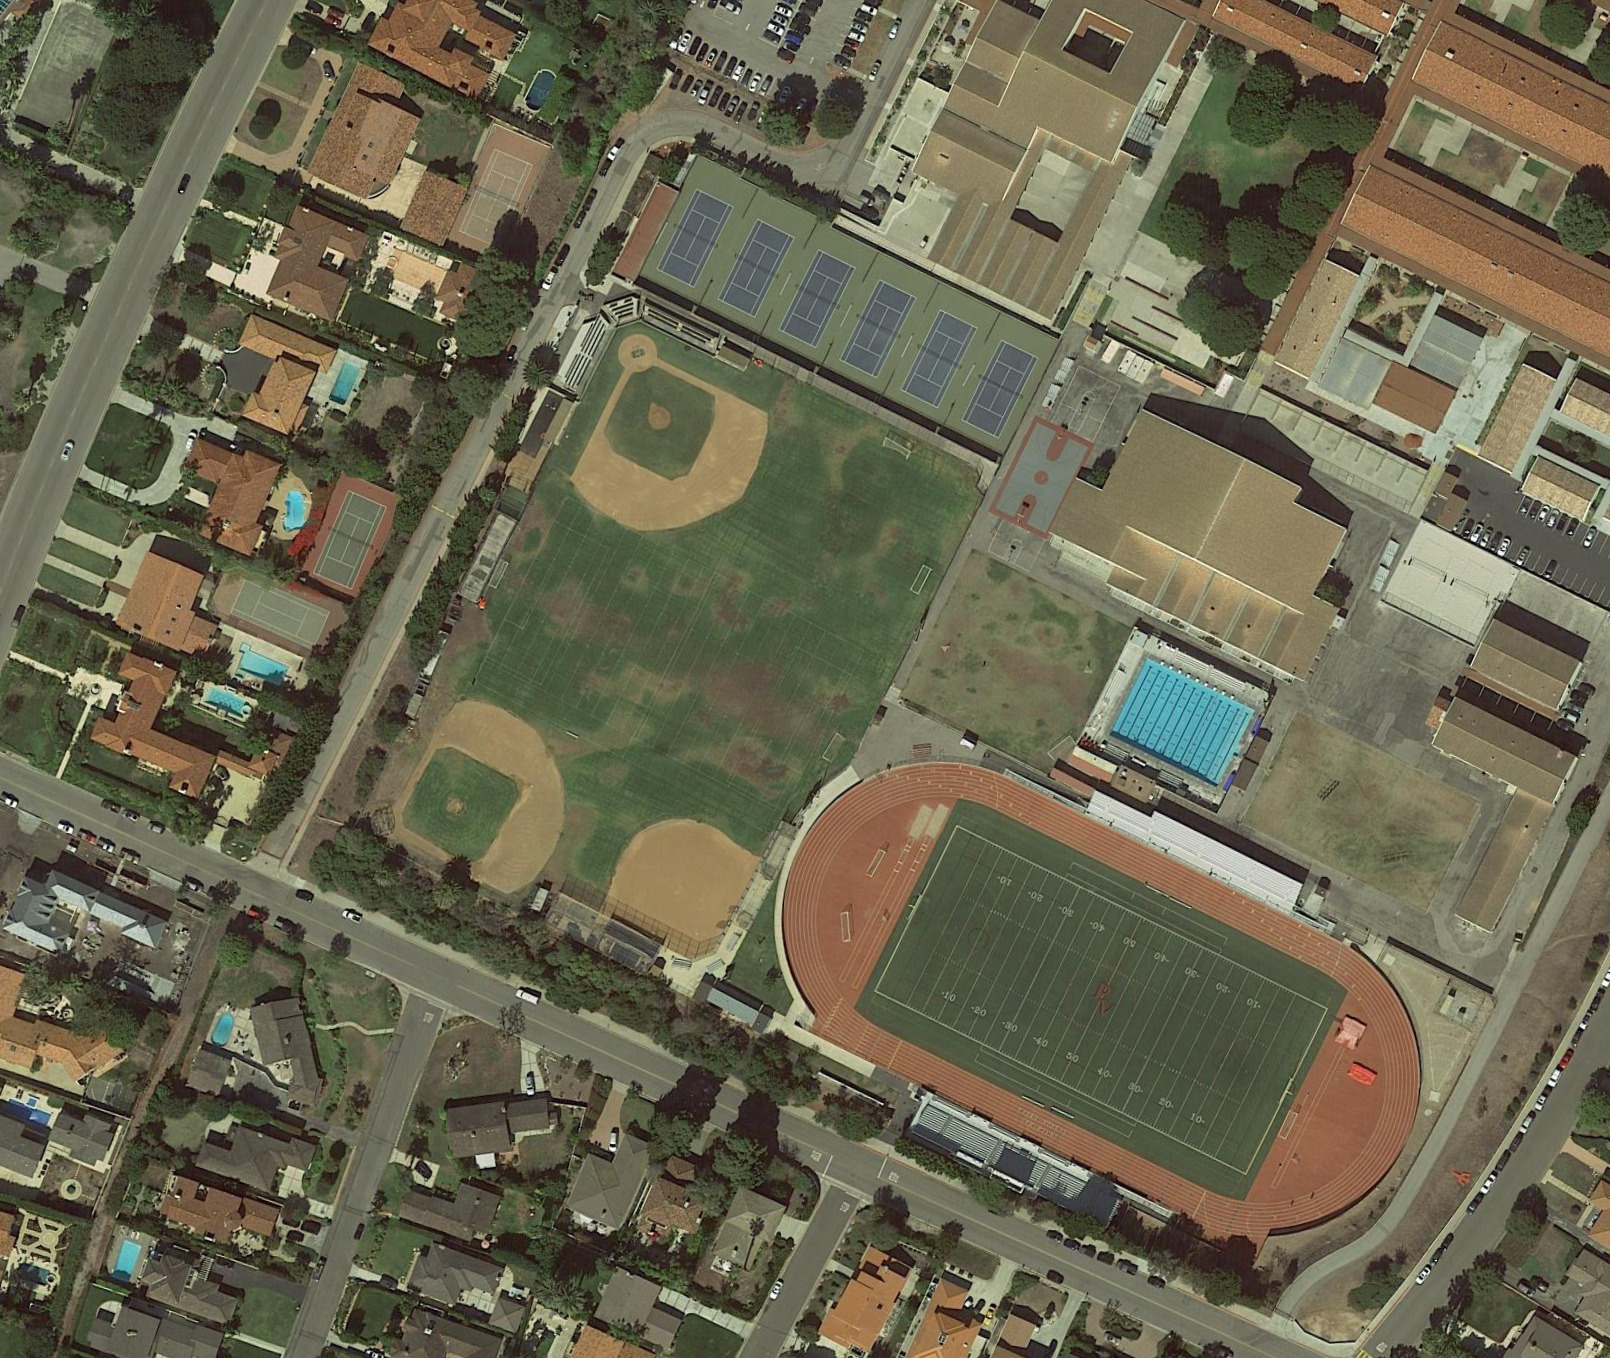
\includegraphics[width=30mm]{Figures/P0770.jpg}
                };
               
            \end{tikzpicture}
            
        \end{column}
        \pause
        
        \begin{column}{0.3\textwidth}
            

            \only<4->{
                \begin{textblock*}{50mm}(41mm,53mm)
                    \huge $\rightarrow$
                \end{textblock*}
                

                \begin{tikzpicture}[remember picture,overlay]
                    \node[xshift=\paperwidth/2 +0mm,yshift=-\paperheight/2- 5mm] at (current page.north west){%
                        \fbox{\parbox[][10mm][c]{0.8\textwidth}{\centering\normalsize Modèle de détection}}
                    };
                \end{tikzpicture}
            }
            % \graphicsbox{Figures/P0131.jpg}{(0.2,0.2)}{(0.23,0.5)}{green}[20mm][0.2mm]
        \end{column}
        \pause
        \begin{column}{0.3\textwidth}
            \only<5->{
                \begin{textblock*}{50mm}(82mm,53mm)
                    \huge $\rightarrow$
                \end{textblock*}
                \centering
                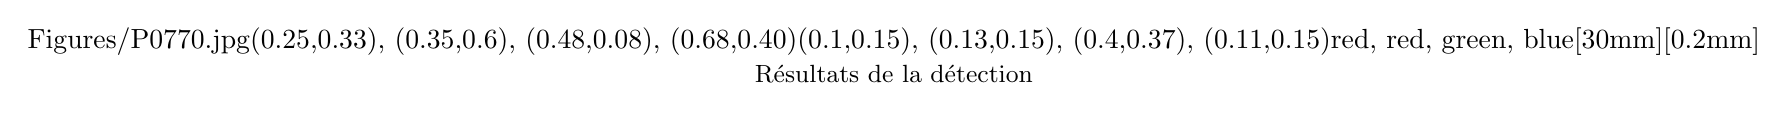
\begin{tikzpicture}
                    \node[anchor=south west,inner sep=0, label=below:{\small Résultats de la détection}] at (0,0){
                        \graphicsbox{Figures/P0770.jpg}{(0.25,0.33), (0.35,0.6), (0.48,0.08), (0.68,0.40)}{(0.1,0.15), (0.13,0.15), (0.4,0.37), (0.11,0.15)}{red, red, green, blue}[30mm][0.2mm]
                    };
                
                \end{tikzpicture}
            }
            
        \end{column}
    \end{columns}
    
    \only<3->{
    \begin{textblock}{12}(2, 12)
        \[ \mathcal{C} = \{ \text{Terrain de baseball, Piscine, Piste d'athlétisme} \}\]
      \end{textblock}
    }
        
\end{subsectionframemod}

    \subsection{Principe de la détection d'objets few-shot}\label{subsec:fs-od-definition}
    \begin{subsectionframemod}{Few-Shot Object Detection}
    \metroset{block=fill}
    \vspace{-10mm}
    \begin{alertblock}{$n$-way $k$-shot object detection}
        Étant donné des exemples de support $\{(x_1, a_1), \dots, (x_{nk}, a_{nk})\}$, il s'agit de détecter toutes les occurrences des classes dans $\mathcal{C}$ ($|\mathcal{C}| = n$) dans une image de requête $x_q$.
    \end{alertblock}

    \vspace{5mm}
    \pause
    \begin{columns}
        \begin{column}{0.3\textwidth}
            \centering
            \begin{tikzpicture}
                \node[anchor=south west,inner sep=0, label=below:{\small Query image}] at (0,0){
                    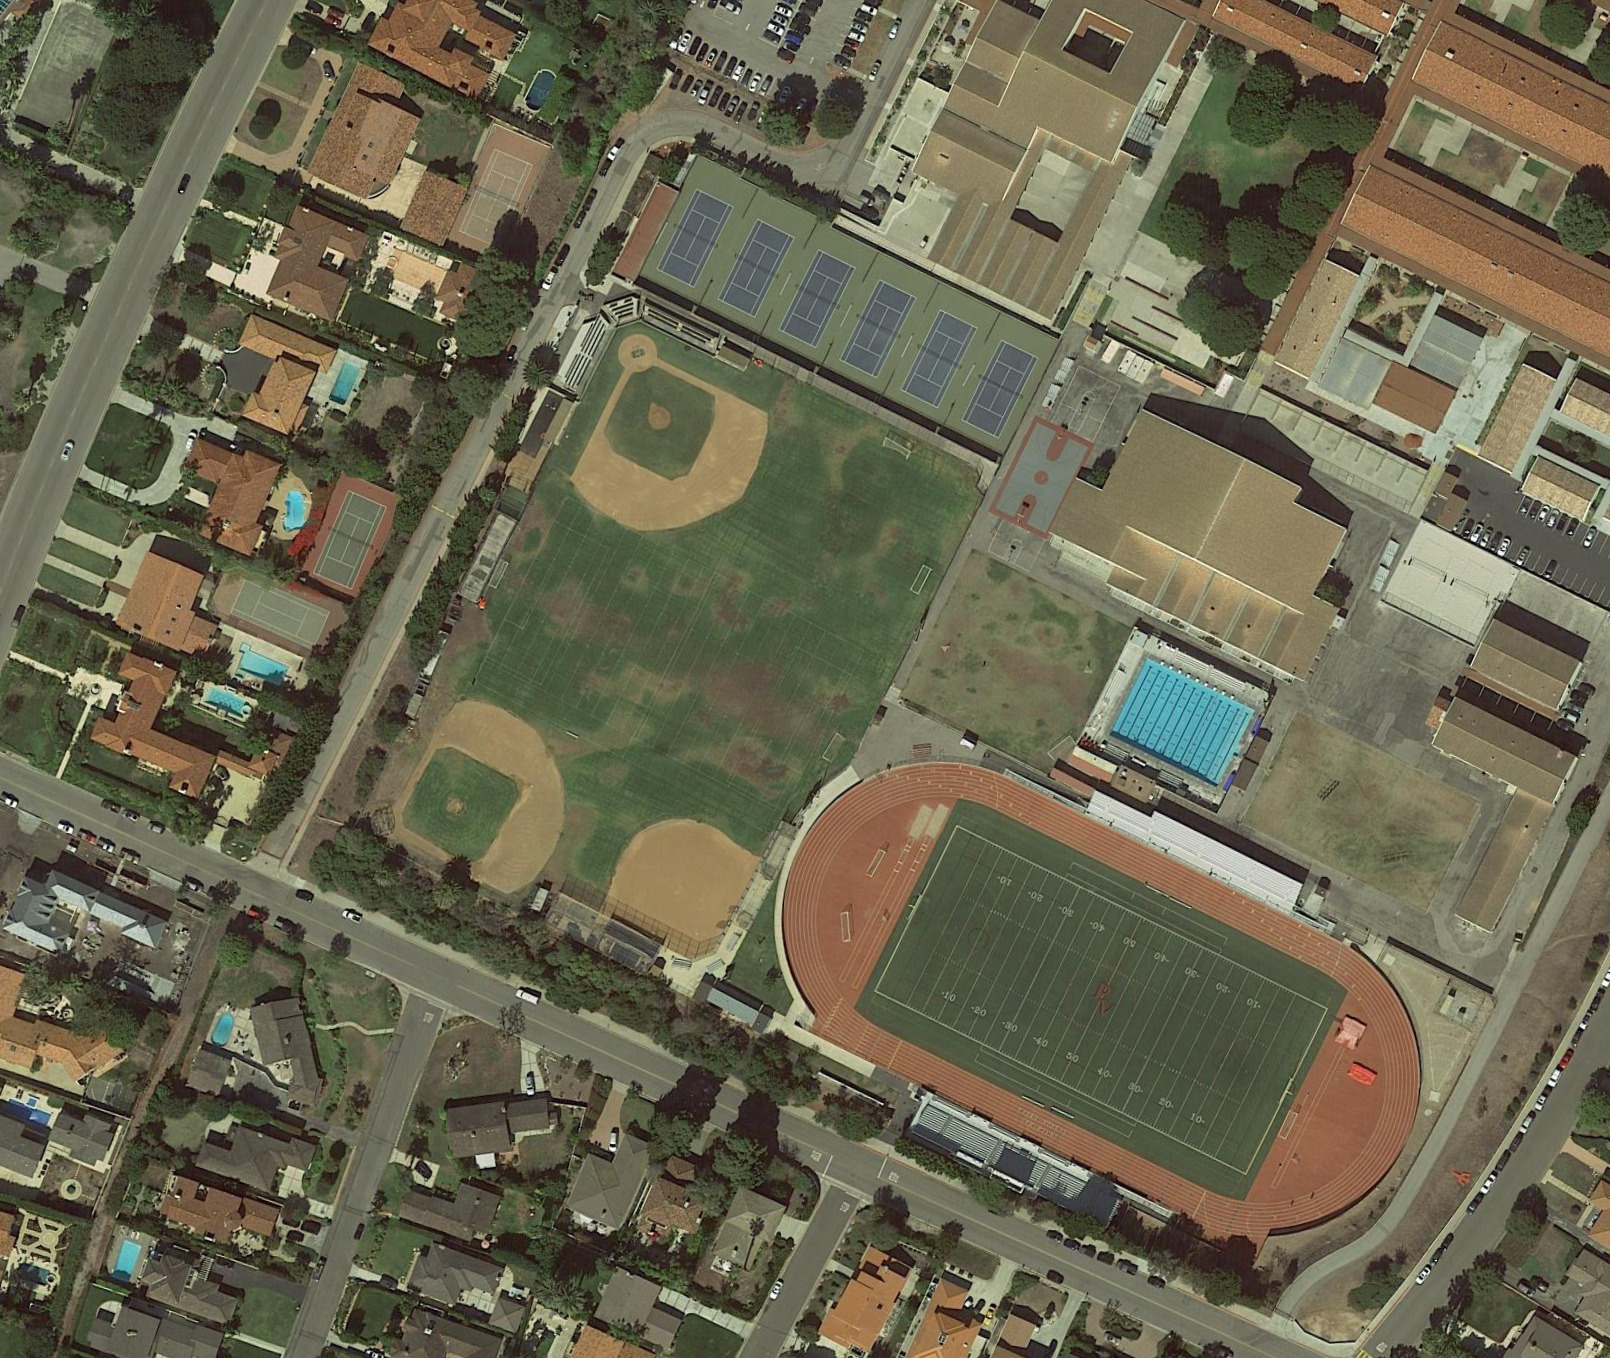
\includegraphics[width=30mm]{Figures/P0770}
                };
               
            \end{tikzpicture}
            
        \end{column}
        \pause
        
        \begin{column}{0.3\textwidth}
            
            \begin{tikzpicture}[remember picture,overlay]
                \only<3->{
                    \node[xshift=\paperwidth/2,yshift=-\paperheight/2-32mm, label=below:{\small Exemples de support}](support) at (current page.north west){%

                    \graphicsbox{Figures/P0131.jpg}{(0.2,0.2)}{(0.23,0.5)}{green}[15mm][0.2mm]
                    \graphicsbox{Figures/P0168.jpg}{(0.26,0.38)}{(0.07,0.07)}{blue}[15mm][0.2mm]
                    \graphicsbox{Figures/P0352.jpg}{(0.6,0.18)}{(0.3,0.3)}{red}[15mm][0.2mm]
                    };
                }
                
                
                \only<4->{\draw[decorate, decoration ={brace,raise=1pt}] (support.north west) -- (support.north east)
                    node (supportlabel) [midway, above=10pt] {\huge $\uparrow$};}

            \end{tikzpicture}
            \only<4->{
                \begin{textblock*}{50mm}(41mm,53mm)
                    \huge $\rightarrow$
                \end{textblock*}
                

                \begin{tikzpicture}[remember picture,overlay]
                    \node[xshift=\paperwidth/2 +0mm,yshift=-\paperheight/2- 5.5mm] at (current page.north west){%
                        \fbox{\parbox[][10mm][c]{0.8\textwidth}{\centering\normalsize Modèle de détection}}
                    };
                \end{tikzpicture}
            }
            % \graphicsbox{Figures/P0131.jpg}{(0.2,0.2)}{(0.23,0.5)}{green}[20mm][0.2mm]
        \end{column}
        \pause
        \begin{column}{0.3\textwidth}
            \only<5->{
                \begin{textblock*}{50mm}(82mm,53mm)
                    \huge $\rightarrow$
                \end{textblock*}
                \centering
                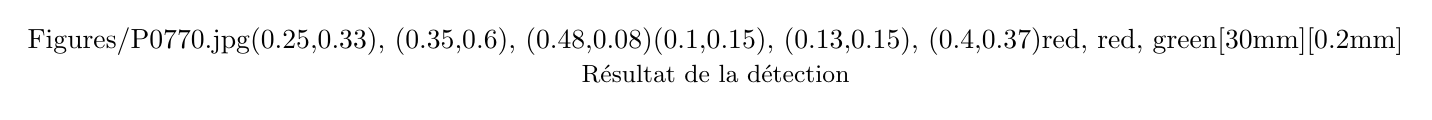
\begin{tikzpicture}
                    \node[anchor=south west,inner sep=0, label=below:{\small Résultat de la détection}] at (0,0){
                        \graphicsbox{Figures/P0770.jpg}{(0.25,0.33), (0.35,0.6), (0.48,0.08)}{(0.1,0.15), (0.13,0.15), (0.4,0.37)}{red, red, green}[30mm][0.2mm]
                    };
                
                \end{tikzpicture}
            }
            
        \end{column}
    \end{columns}
        
\end{subsectionframemod}

%    \subsection{Introduction - Challenges de la détection d'objets few-shot sur les images aériennes}\label{sec:fs-od-challenges}
%    \begin{subsectionframemod}{Difference between Natural and Aerial Images}
    La plupart des méthodes sont évaluées sur des images naturelles : les ensembles de données Pascal VOC et MS COCO.
    $\Rightarrow$ cela ne garantit pas de bonnes performances sur les images aériennes.
    \vspace{2mm}


    Les tailles des objets sont extrêmement différentes entre les images aériennes et naturelles.

    \begin{figure}
        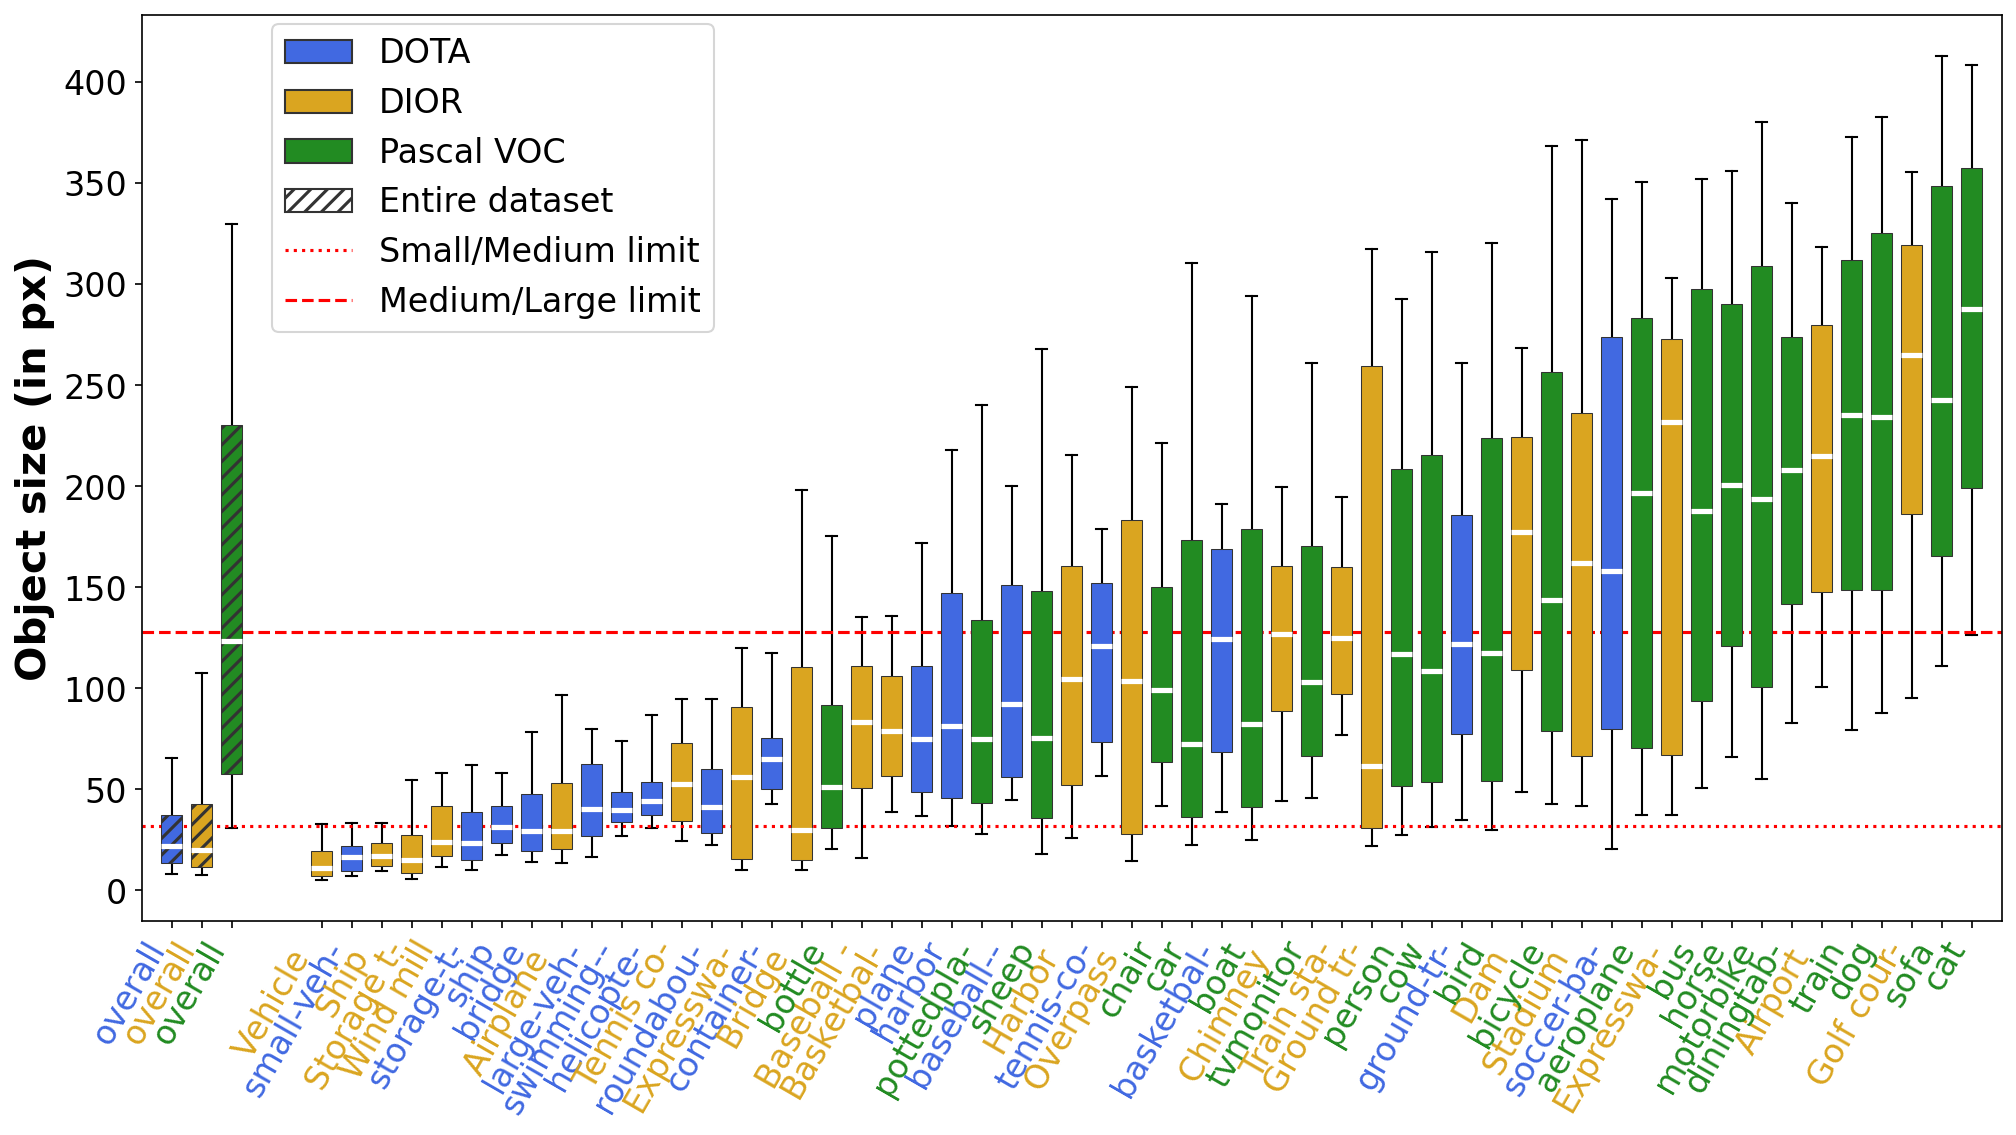
\includegraphics[width=0.8\textwidth]{Figures/object_sizes.png}
    \caption{Diagramme en boîte des tailles d'objets dans DOTA (\cite{xia2018dota}), DIOR (\cite{li2020object}) et Pascal VOC (\cite{everingham2010pascal}); par classe \textbf{(à droite)} et globalement \textbf{(à gauche)}.}
    \end{figure}

    

    
\end{subsectionframemod}
%    \begin{subsectionframemod}{Performance Analysis}
    
    
    Il est impossible de comparer les performances sur différents ensembles de données.
    Cependant, il est possible de \alert{comparer les performances FSOD par rapport à une référence non few-shot}
    et de comparer cela sur plusieurs ensembles de données.

    \begin{figure}
        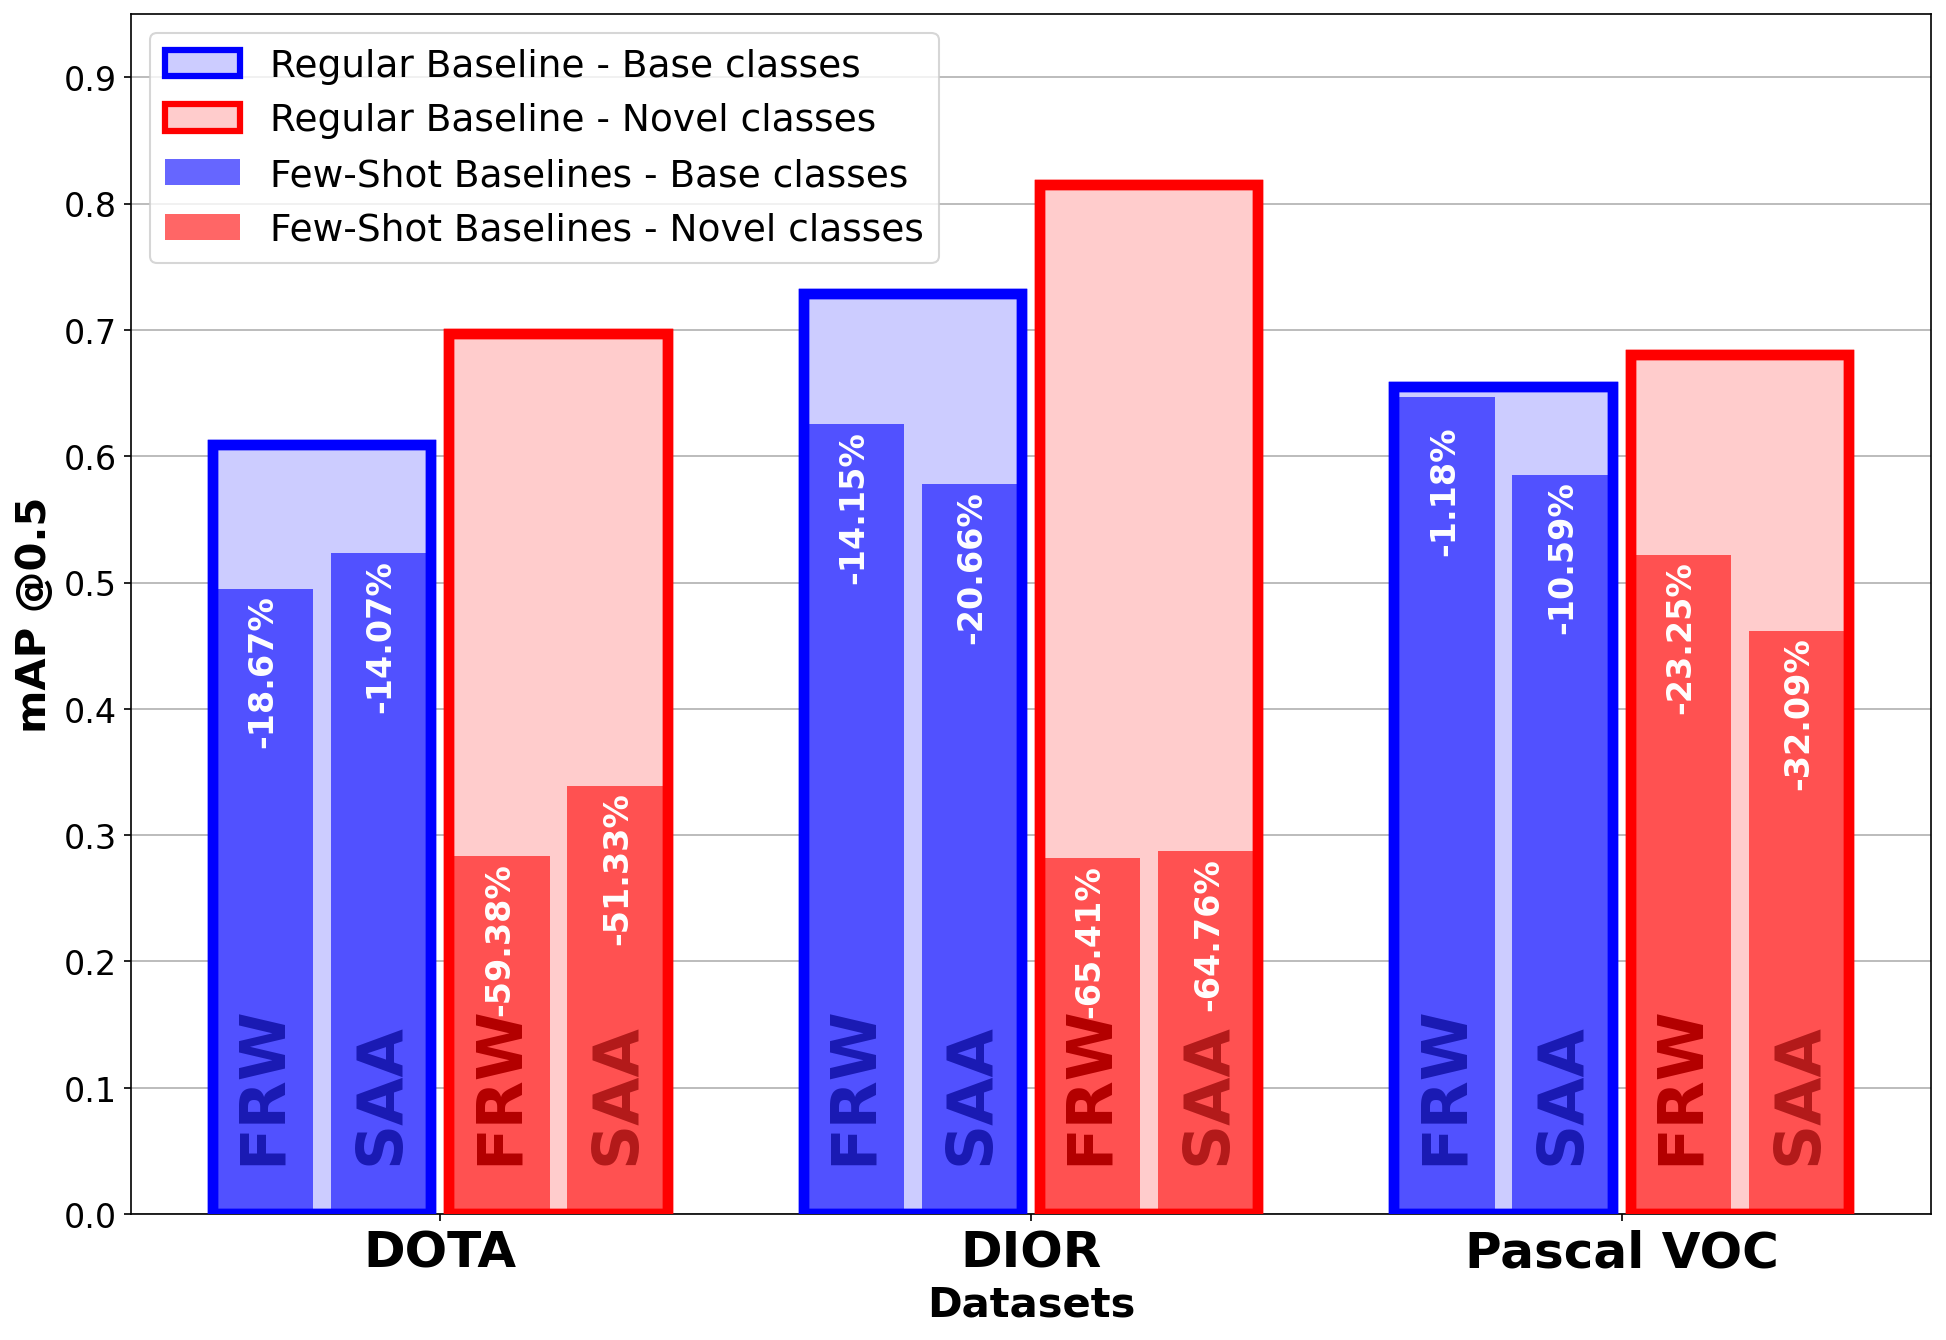
\includegraphics[width=0.8\textwidth]{Figures/dataset_comparison.png}
        \caption{Performances FSOD comparées sur DOTA, DIOR et Pascal VOC. (\cite{lejeune2022improving})}
    \end{figure}

\end{subsectionframemod}

\begin{subsectionframemod}{Performance Analysis}
    Les grandes différences de taille moyenne entre les classes suggèrent d'analyser les performances par classe.
    \alert{Corrélation claire entre la taille moyenne des classes et les performances} par rapport à la référence.
    \begin{figure}
        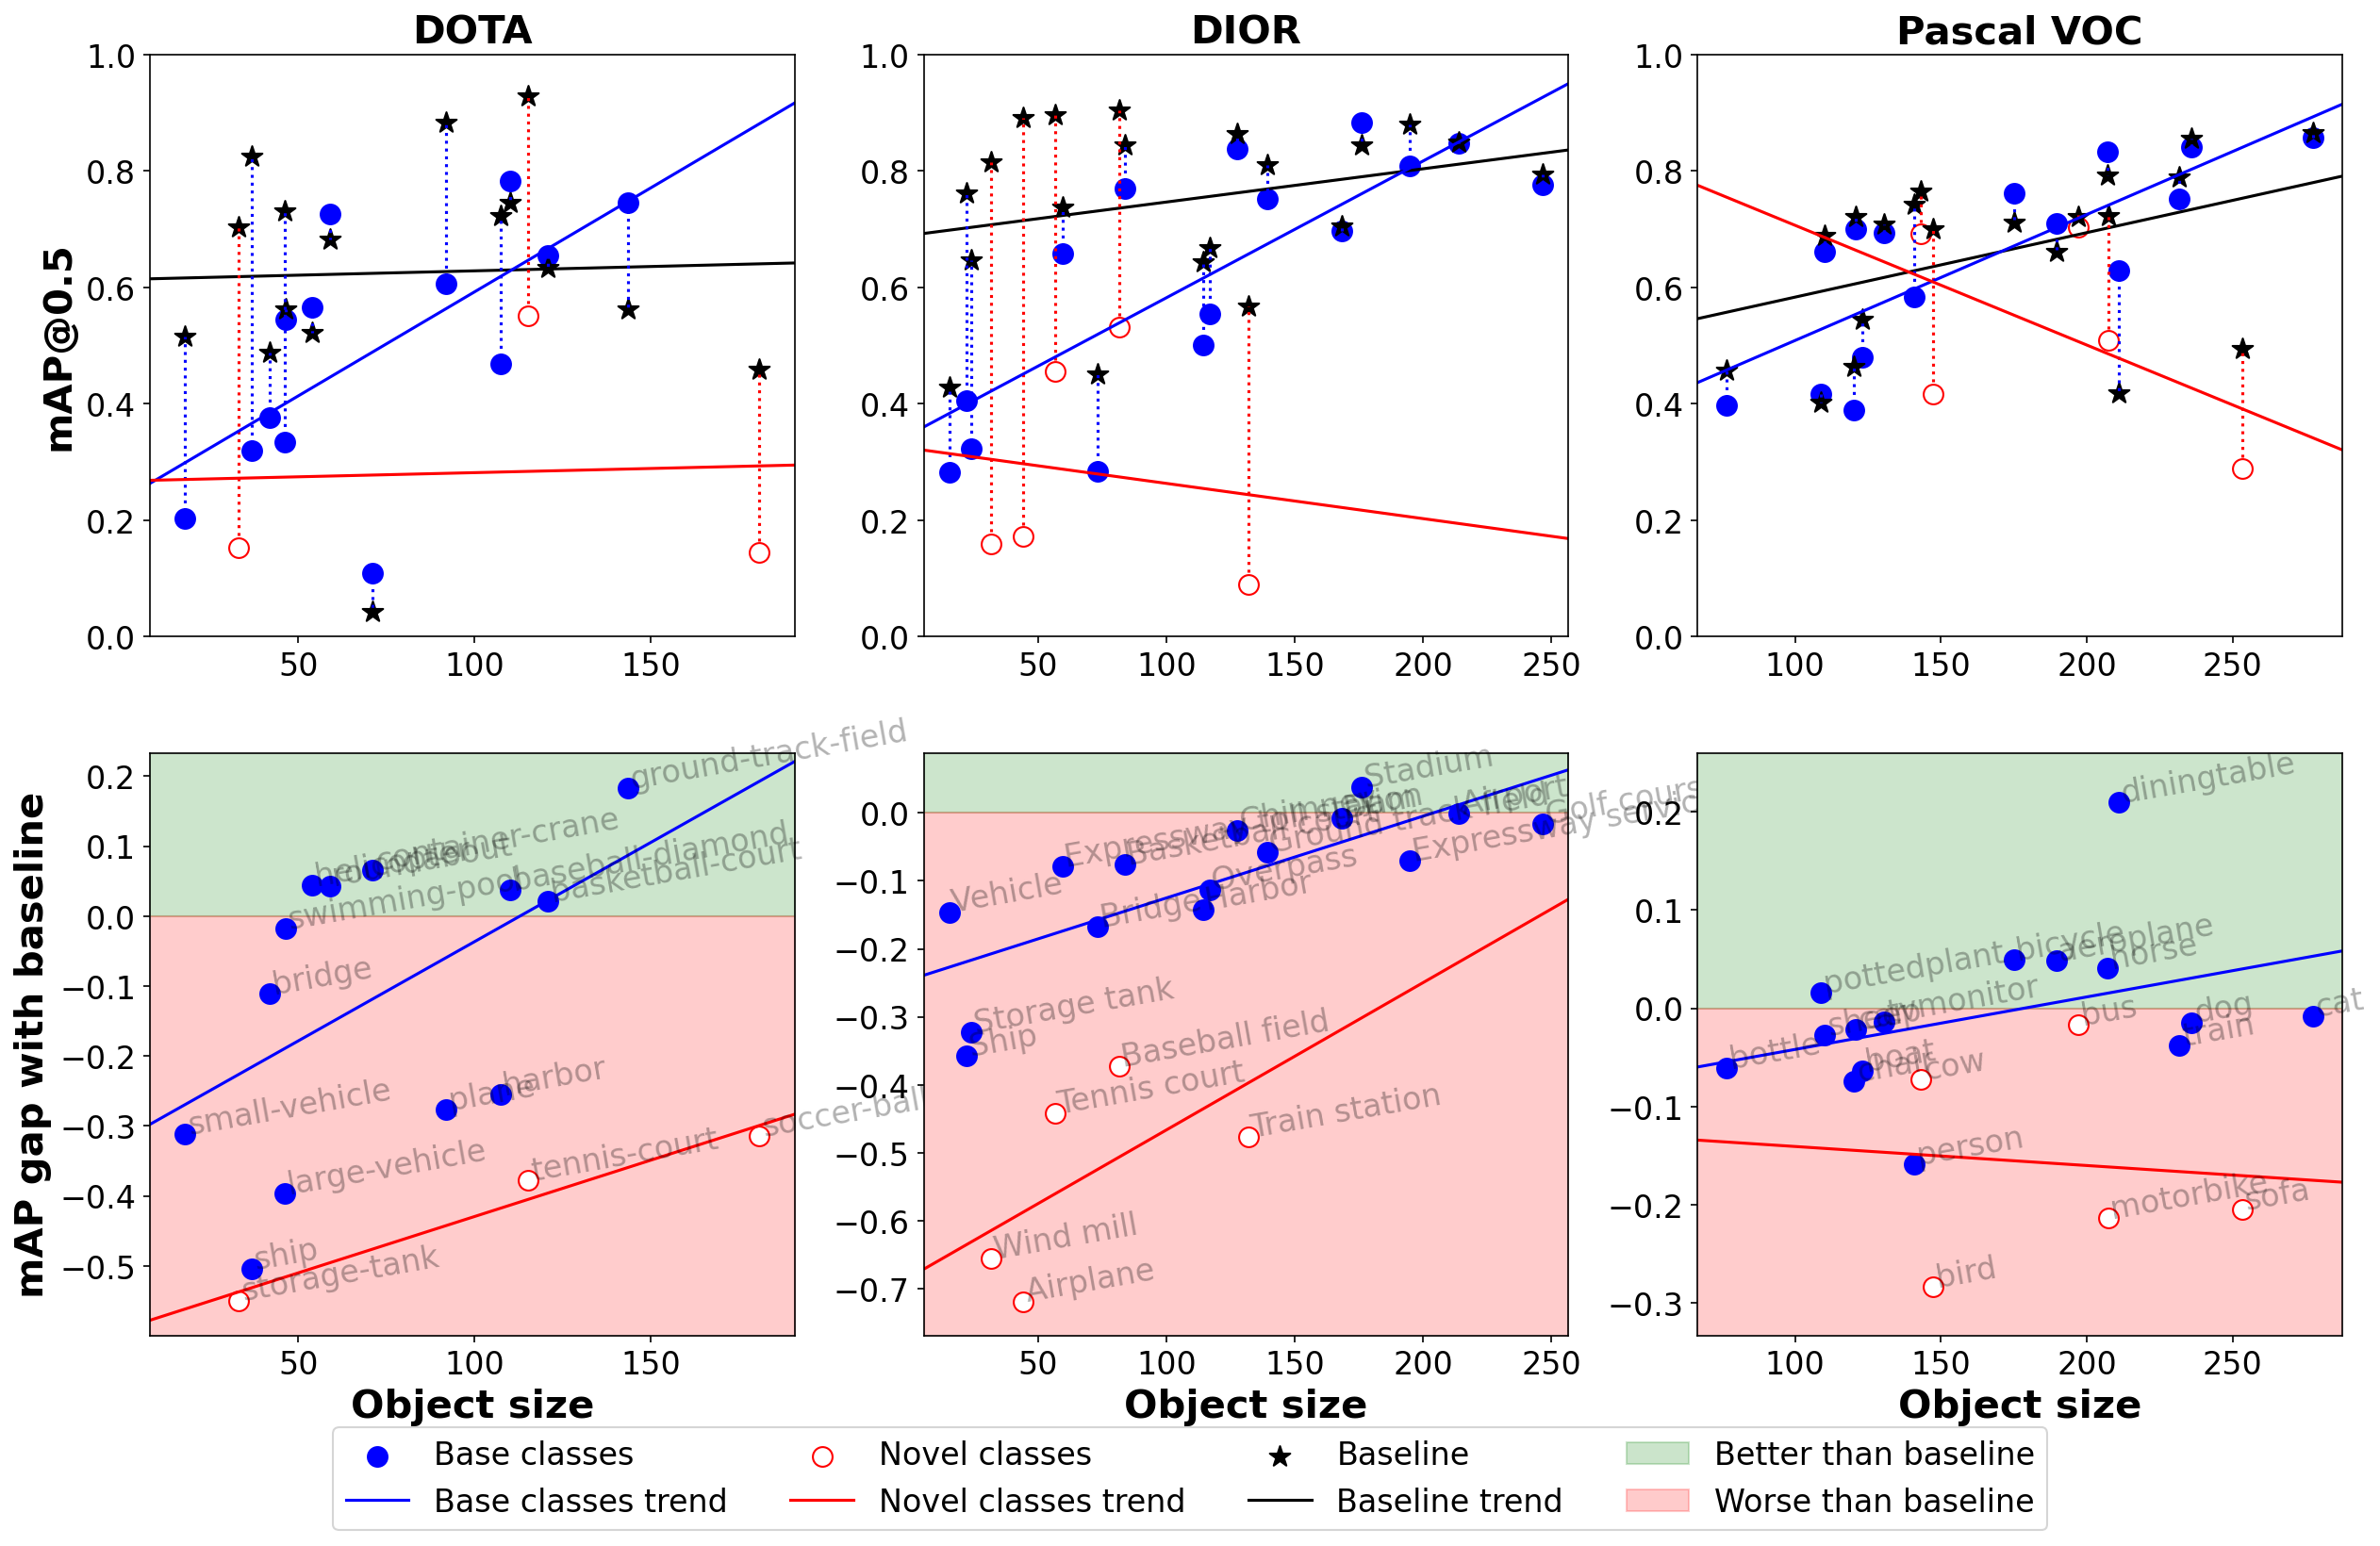
\includegraphics[width=0.85\textwidth]{Figures/performance_comparison.png}
    \caption{Analyse des performances par classe et comparaison avec la référence non few-shot sur DOTA, DIOR et Pascal VOC. (\cite{lejeune2022improving})}
    \end{figure}

\end{subsectionframemod}

    \section{Étude et analyse des performances de la détection d'objets few-shot cross-domain}\label{subsec:fs-od-cd}
    \subsection{Principe de la détection d'objets few-shot cross-domain}\label{subsec:fs-od-cd-principle}
    \begin{subsectionframemod}{Cross-Domain Few-Shot Object Detection}

    \metroset{block=fill}
    \begin{alertblock}{Détection d'objets few-shot cross-domain}
        Dans la détection d'objets few-shot cross-domain, on dispose de deux datasets de deux domains distincts.
        L'un est composé d'un grand nombre de données annotées (le dataset source) tandis que l'autre est plutôt limité (le dataset cible).
        L'objectif est de s'aider du dataset source pour réaliser la détection sur le dataset cible.
        Le modèle doit dans ce cas s'adapter à la fois à de nouvelles classes et à de nouvelles images ce qui complexifie la tâche.
    \end{alertblock}

    \only<1>{
        \begin{figure}
            \centering
            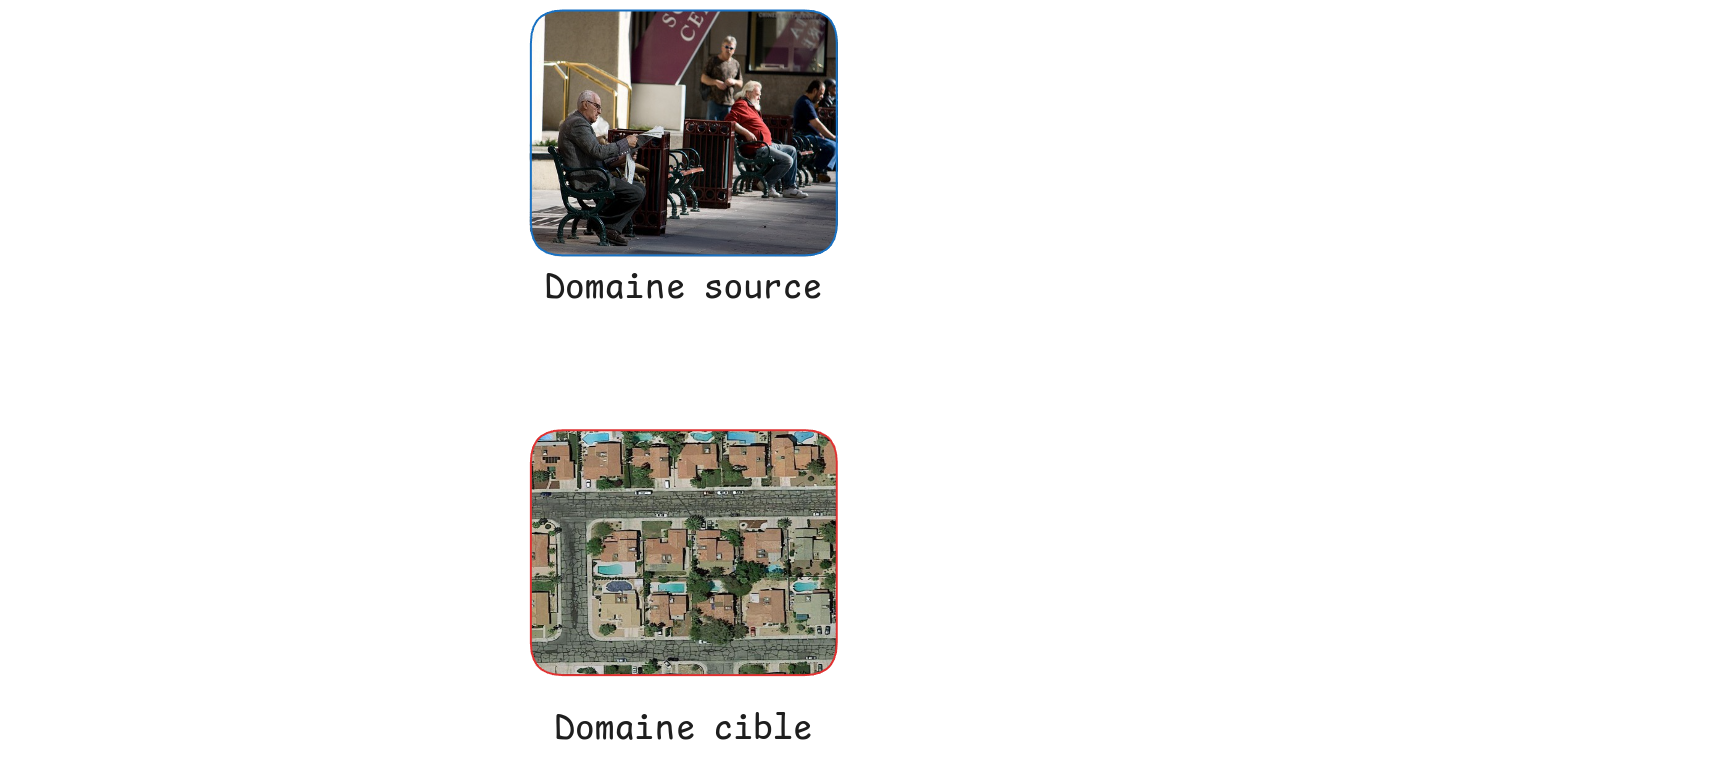
\includegraphics[width=\textwidth]{Figures/cross_domain}
        \end{figure}
    }
    \pause
    \only<2>{
        \begin{figure}
            \centering
            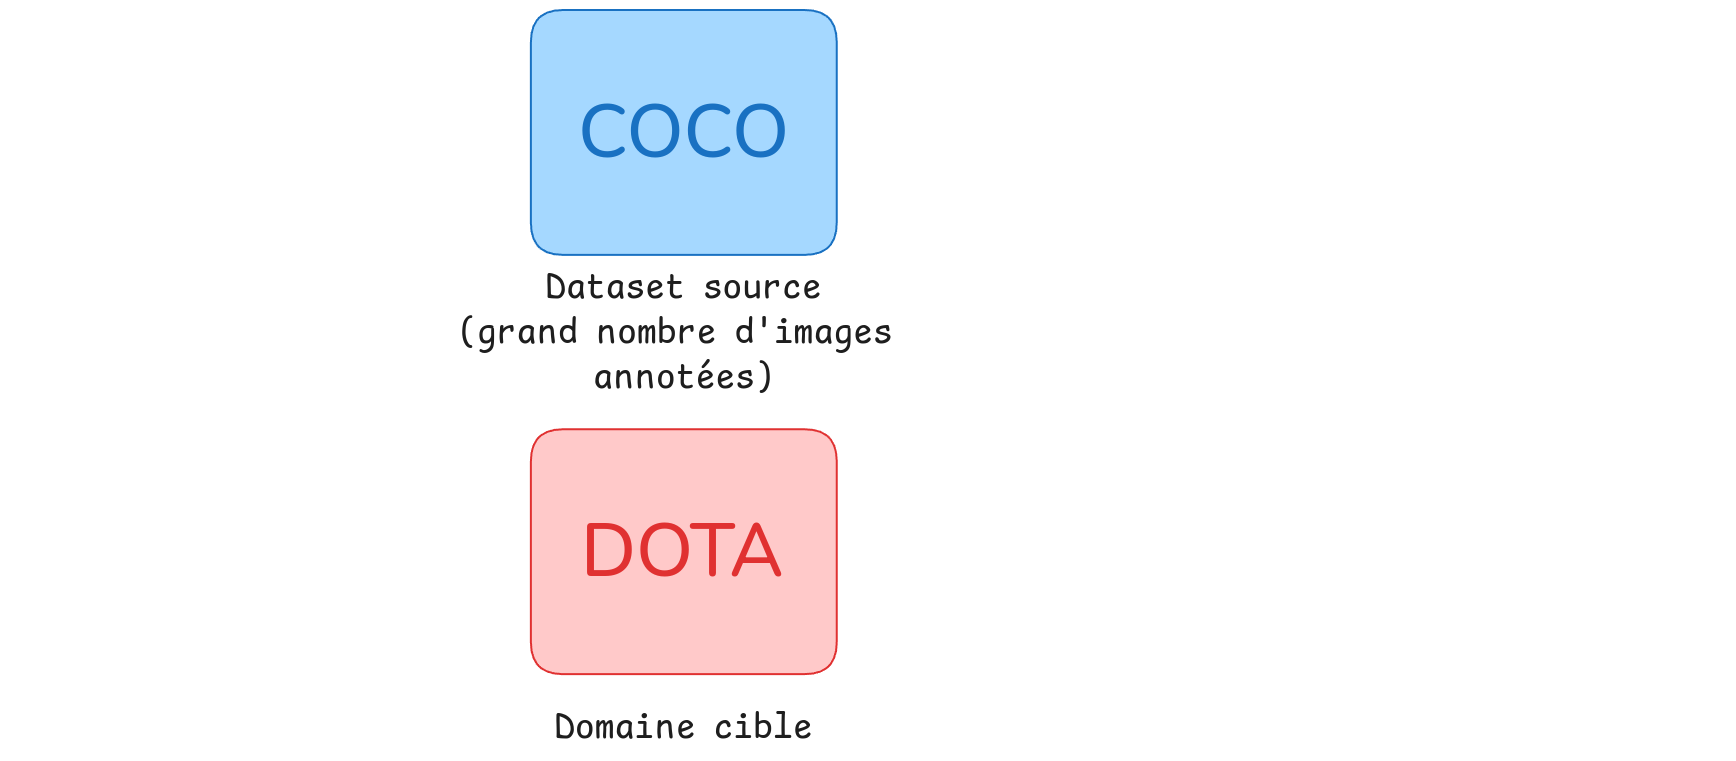
\includegraphics[width=\textwidth]{Figures/cross_domain_0}
        \end{figure}
    }
    \pause
    \only<3>{
        \begin{figure}
            \centering
            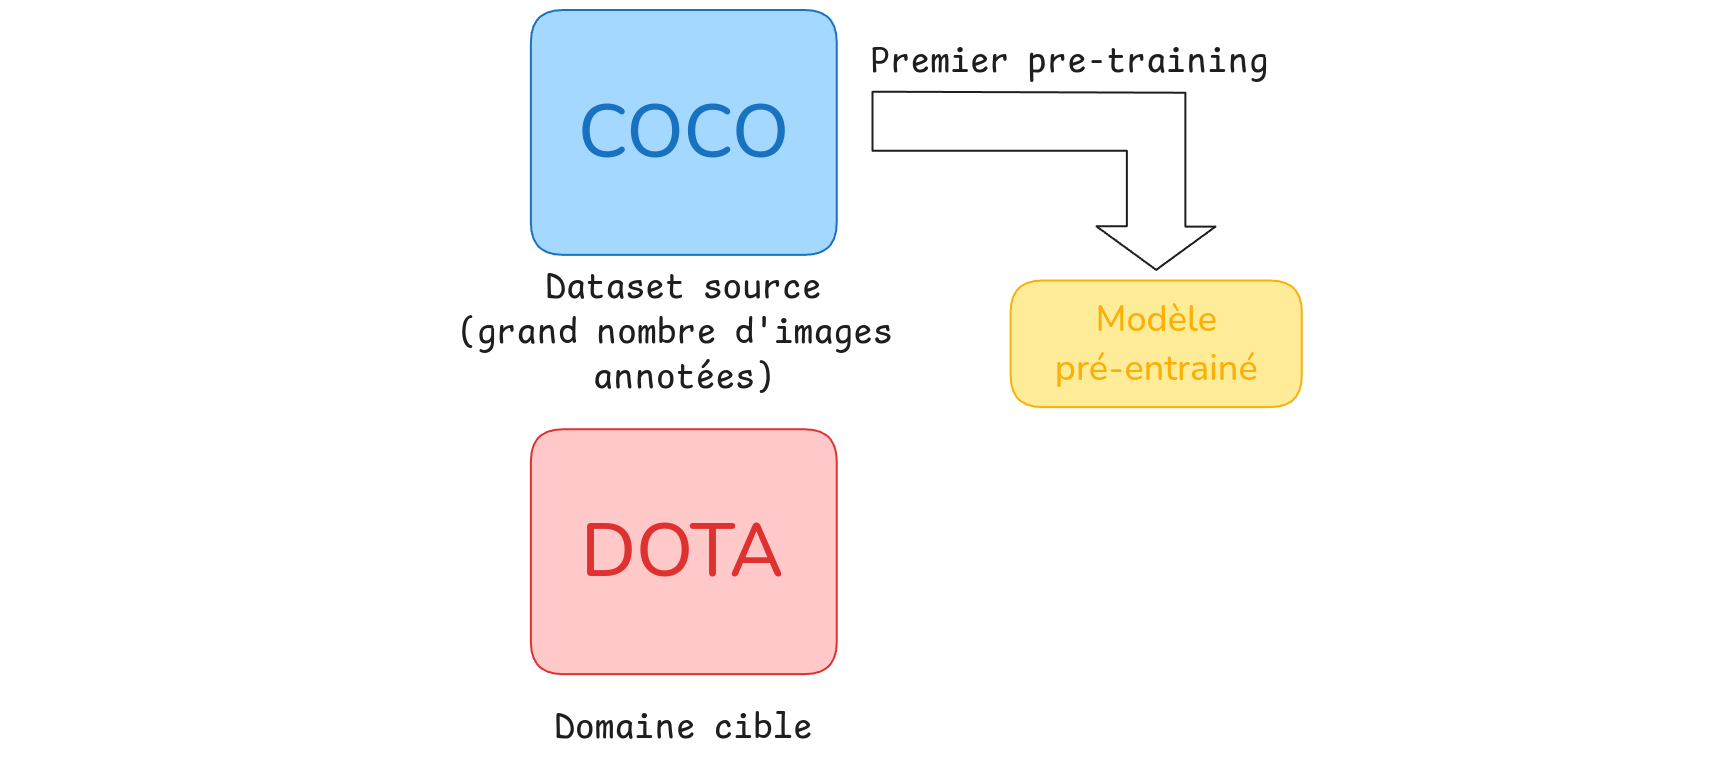
\includegraphics[width=\textwidth]{Figures/cross_domain_1}
        \end{figure}
    }
    \pause
    \only<4>{
        \begin{figure}
            \centering
            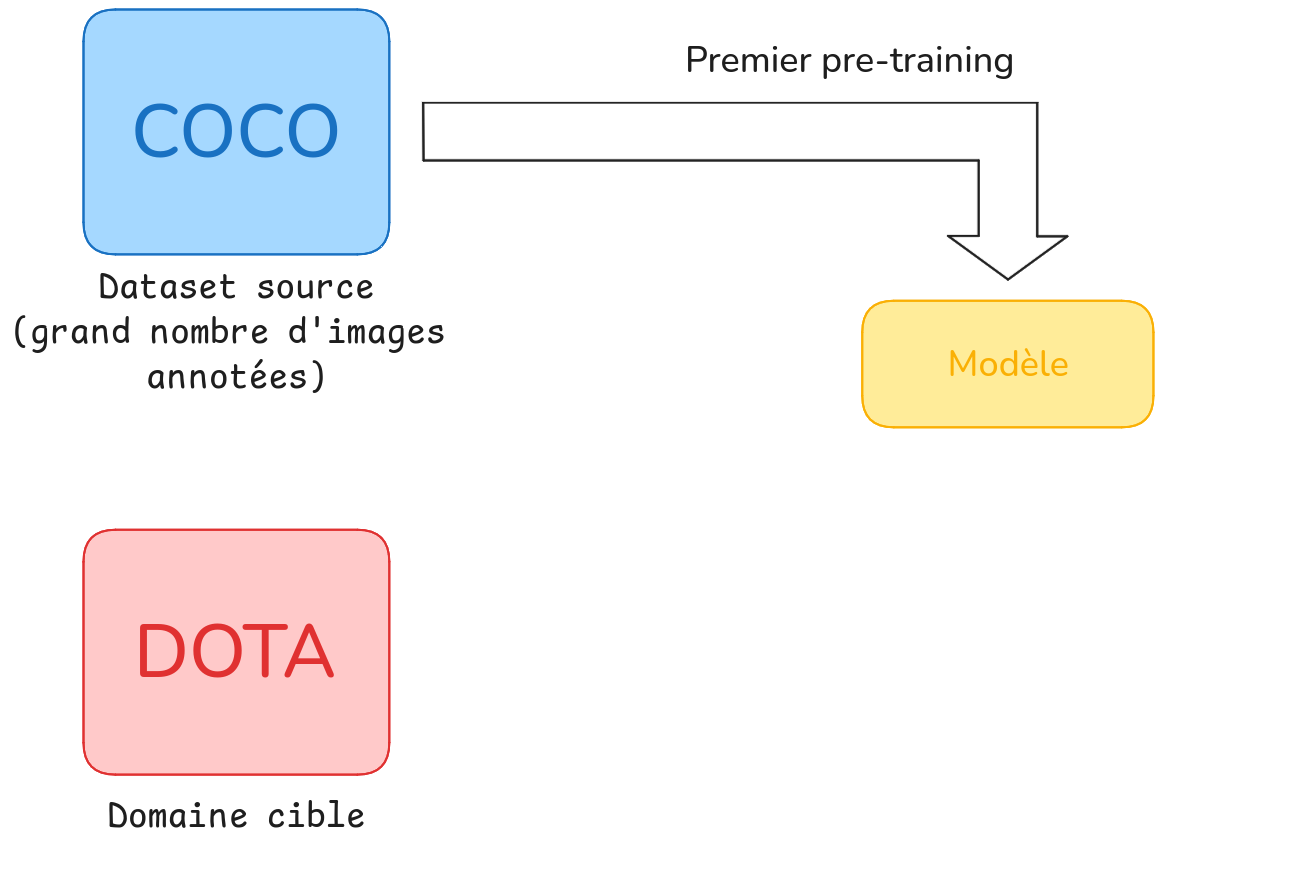
\includegraphics[width=\textwidth]{Figures/cross_domain_2}
        \end{figure}
    }
    \pause
    \only<5>{
        \begin{figure}
            \centering
            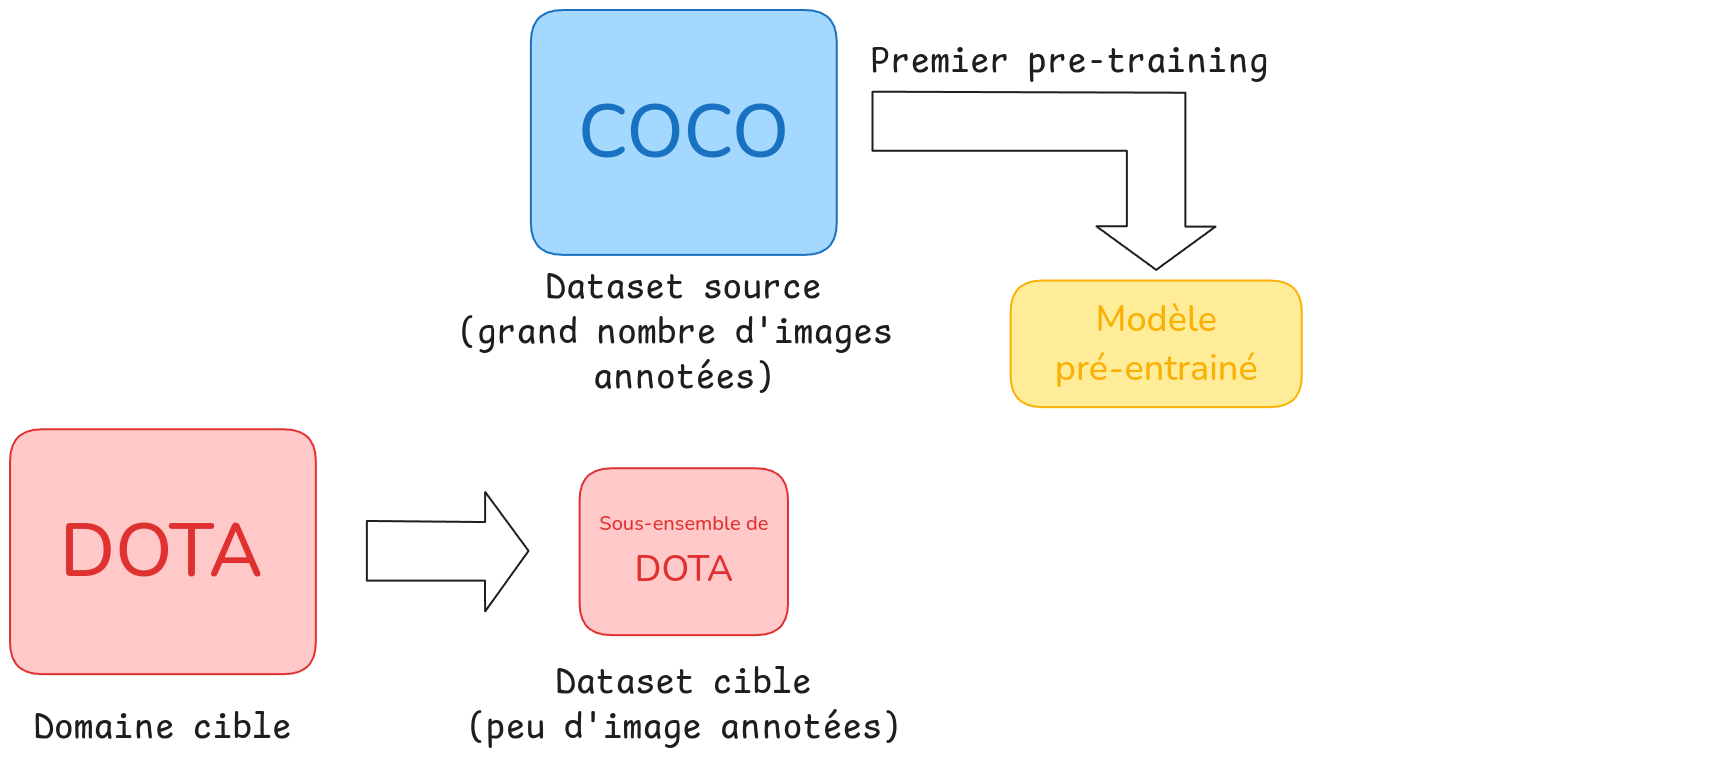
\includegraphics[width=\textwidth]{Figures/cross_domain_3}
        \end{figure}
    }
    \pause
    \only<6>{
        \begin{figure}
            \centering
            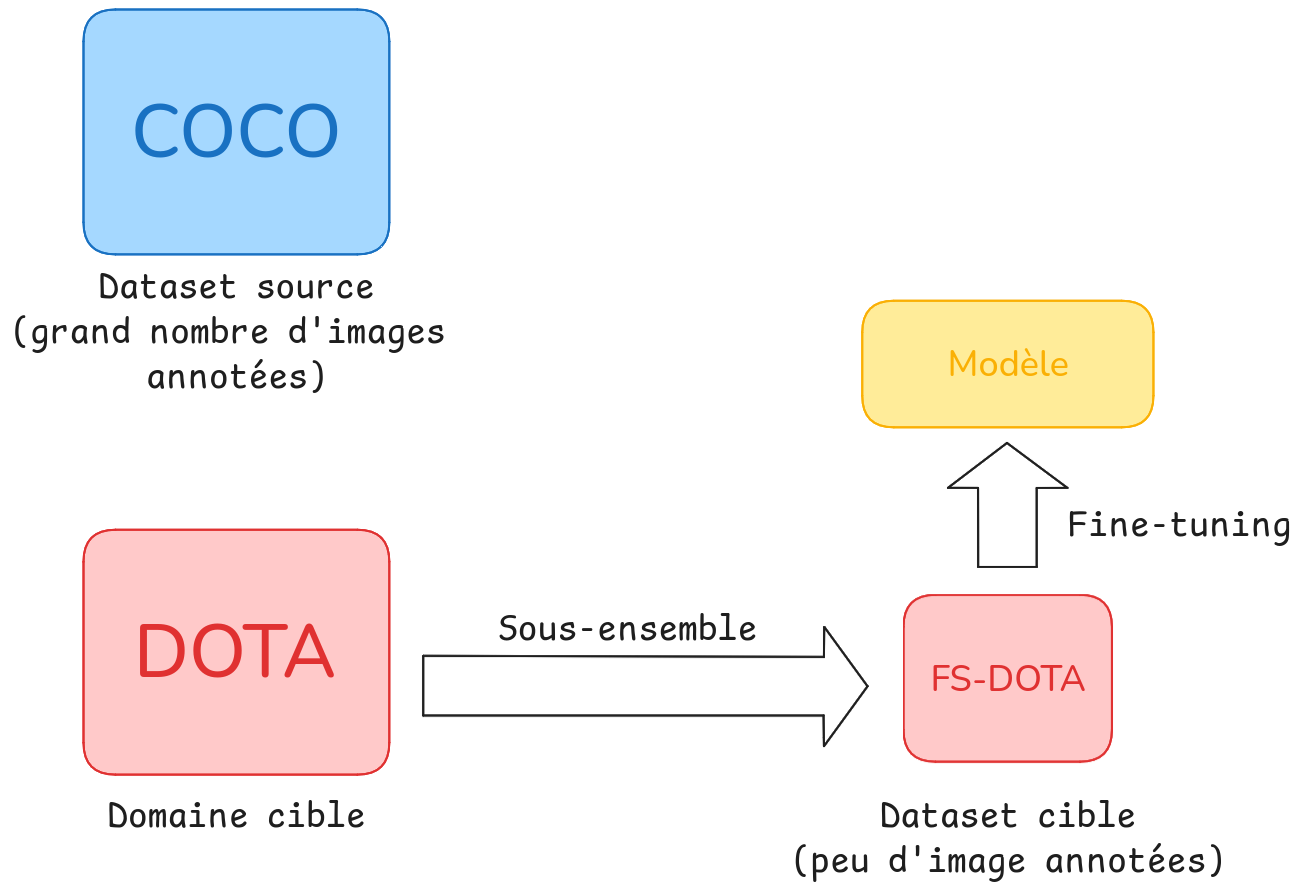
\includegraphics[width=\textwidth]{Figures/cross_domain_4}
        \end{figure}
    }

\end{subsectionframemod}
    \subsection{Principaux travaux réaliser pour répondre aux problèmes de la détection d'objets few-shot cross-domain}\label{subsec:fs-od-cd-research}
    \begin{subsectionframemod}{Publications}
    \textbf{Les recherches effectuées au cours de l'année ce sont articulés autours de 3 axes de recherche principaux :}
    \begin{itemize}
        \item[-] Le developpement d'un framework permettant de comparer rapidement et efficacement les performances des modèles les plus performants aujourd'hui.
        \item[-] La mise en valeur de l'importance du choix d'un bon dataset source, puis l'estimation de l'écart entre domaines permettant de prédire le dataset source le plus adapté.
        \item[-] Limité le risque d'overfitting pour assurer une meilleure généralisation des modèles permettant d'améliorer les performances.
    \end{itemize}

\end{subsectionframemod}


    \subsection{Listes des méthodes de détection d'objets pouvant être utilisé en cross-domain}\label{subsec:fs-od-cd-sota}
    \begin{subsectionframemod}{Détection d'objets few-shot}

    \vspace{-3mm}
    \begin{table}[h]

    \label{tab:comparison}
    \begin{adjustbox}{width=0.75\textwidth}
        \rowcolors{2}{gray!25}{white}
        % \begin{tabular}{lllTLLT}
        \begin{tabular}{@{}lc}
            \begin{tabular}{@{}lc}
                \toprule[1pt]
                \textbf{Name}                               & \textbf{Backbone} \\ \hline
                Meta-RCNN~\parencite{wu2020meta}            & ResNet50          \\
                TFA w/cos~\parencite{wang2020frustratingly} & ResNet50          \\
                FSCE~\parencite{sun2021fsce}                & ResNet50          \\
                DeFRCN~\parencite{qiao2021defrcn}           & ResNet50          \\
                Distill-cdfsod~\parencite{xiong2023cd}      & ResNet50          \\ \hline
                ViTDeT-FT~\parencite{li2022exploring}       & ViT-B/14          \\ \hline
                Detic~\parencite{zhou2022detecting}         & ViT-L/14          \\
                Detic-FT~\parencite{zhou2022detecting}      & ViT-L/14          \\
                DE-ViT~\parencite{zhang2024detect}          & ViT-L/14          \\
                DE-ViT-FT~\parencite{zhang2024detect}       & ViT-L/14          \\
                CD-ViTO~\parencite{fu2024crossdomain}       & ViT-L/14          \\\bottomrule[1pt]
            \end{tabular}%
        \end{tabular}%
    \end{adjustbox}
    \caption{Comparaison des méthodes FSOD du point de vue de l'attention. Tous les
    cadres fonctionnent avec des caractéristiques multiscalaires, sauf celui avec la
    mention sans FPN.}

\end{table}
\end{subsectionframemod}

%\begin{subsectionframemod}{Détection d'objets few-shot}
%
%    \vspace{-3mm}
%    \begin{table}[h]

    \label{tab:comparisonfscd}
    \begin{adjustbox}{width=0.75\textwidth}
        \rowcolors{2}{gray!25}{white}
        % \begin{tabular}{lllTLLT}
        \begin{tabular}{@{}lc}
            \begin{tabular}{@{}lcc}
                \toprule[1pt]
                & \textbf{DOTA} & \textbf{DIOR} \\ \hline
                Few-shot              & 60.45         & 57.51         \\ \hline
                Cross-domain Few-shot (COCO) & 25.02         & 38.73         \\
                Cross-domain Few-shot (DOTA) & \_         & 38.44         \\
                Cross-domain Few-shot (DIOR) & 33.30         & \_         \\\bottomrule[1pt]
            \end{tabular}%
        \end{tabular}%
    \end{adjustbox}
    \caption{Comparaison des performances de DiffusionDet (\cite{chen2022diffusiondet}) en Few-shot et en Cross-domain Few-shot sur DOTA et DIOR en considérant 3 dataset source (notés entre paranthèse) avec 10 shots.
    Les performances sont évaluées en mAP (\%) rapporté avec un seuil IoU à 0.5.}

\end{table}
%\end{subsectionframemod}


    \subsection{Etude et analyse de l'impact du dataset source sur les performances des modèles de détection d'objets few-shot cross-domain}\label{subsec:srcdata}
    \begin{subsectionframemod}{Détection d'objet few-shot}
    \metroset{block=fill}

    \begin{alertblock}{Importance of source dataset in cross-domain}
        Le choix du dataset source dans la détection d'objets cross-domain est crucial,
        car il affecte directement la capacité du modèle à se généraliser à de nouveaux domaines cibles non vus.
    \end{alertblock}

    \begin{table}[]
    \centering
    \resizebox{0.9\columnwidth}{!}{%
        \begin{tabular}{@{\hspace{2mm}}cccccccccc@{\hspace{2mm}}}
            \toprule
            \textbf{$k$ shots} & \textbf{DOTA $\to$ DIOR} & & \textbf{COCO $\to$ DIOR} & & \textbf{DIOR $\to$ DOTA} & & \textbf{COCO $\to$ DOTA}      \\ \midrule
            \textbf{1}         & 9.40                     & & \textbf{11.10}           & & \textbf{5.09}            & & 4.03                     \\
            \textbf{5}         & 29.57                    & & \textbf{30.42}           & & \textbf{24.90}           & & 14.45                    \\
            \textbf{10}        & 38.44                    & & \textbf{38.73}           & & \textbf{33.30}           & & 25.02                    \\
            \textbf{20}        & 45.36                    & & \textbf{48.23}           & & \textbf{41.30}           & & 33.31                    \\
            \textbf{50}        & 53.51                    & & \textbf{56.97}           & & \textbf{49.22}           & & 43.23                    \\ \bottomrule[1pt]
        \end{tabular}%
    } \caption{\textcolor{red}{Need a good caption here}}
    \label{tab:cd_fsod_dota2dior}
    \vspace{-1.5em}
\end{table}
\end{subsectionframemod}



    \subsection{Estimation de l'écart entre domaines}\label{subsec:results-variances}
    \begin{subsectionframemod}{Cross-Domain Few-Shot Object Detection}

    \only<1>{
        \begin{figure}
            \centering
            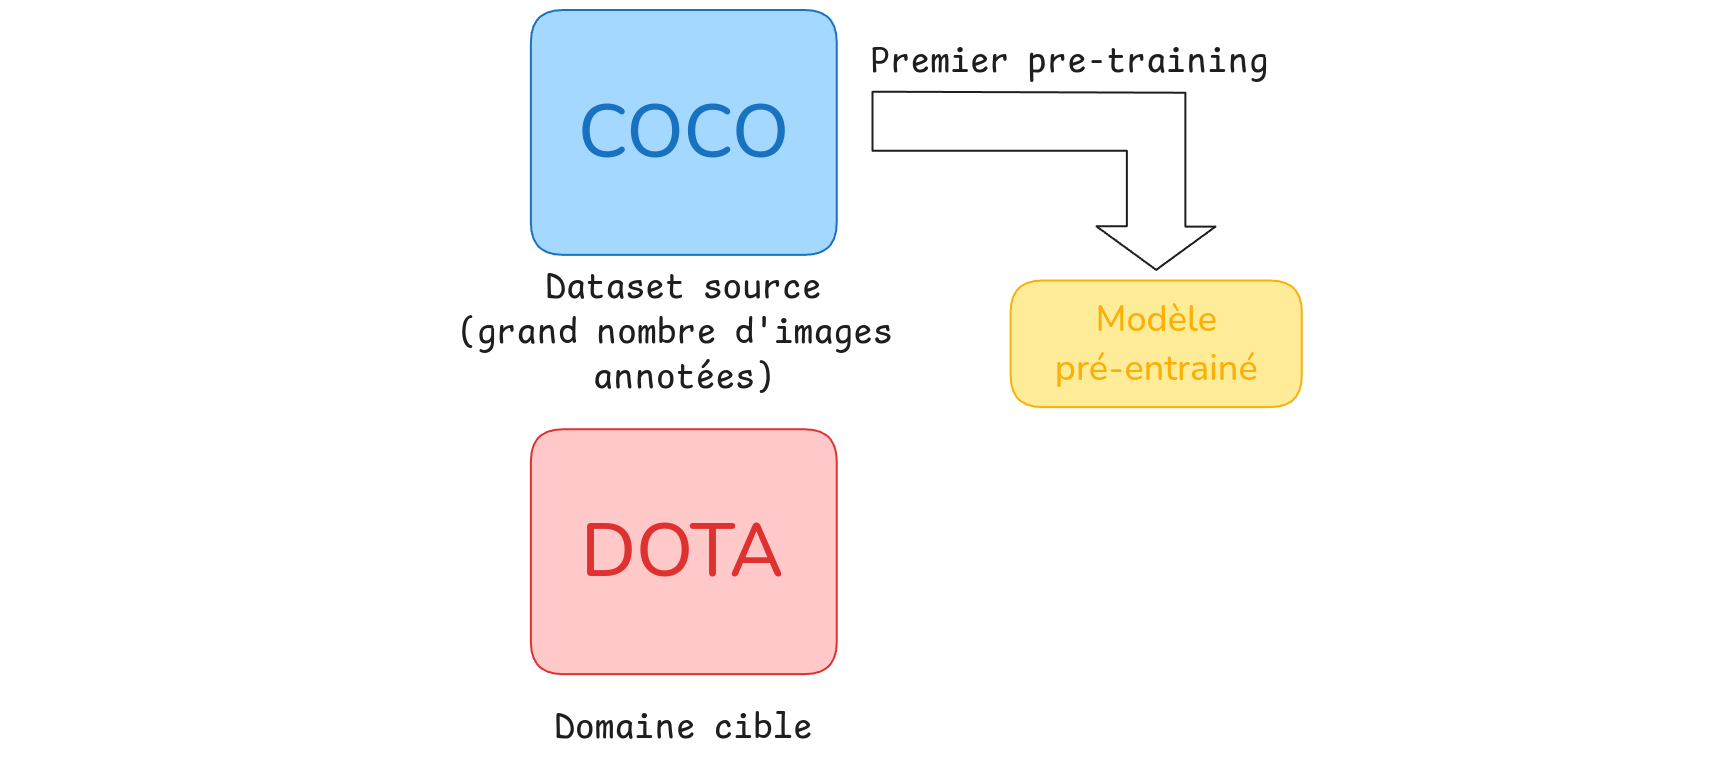
\includegraphics[width=\textwidth]{Figures/cross_domain_1}
            \caption{Méthode utilisée pour extraire le vecteur des caractéristiques.
            L'idée est de remplacer la tête de classification par un module ROI pooling.}
        \end{figure}
    }
    \pause
    \only<2>{
        \begin{figure}
            \centering
            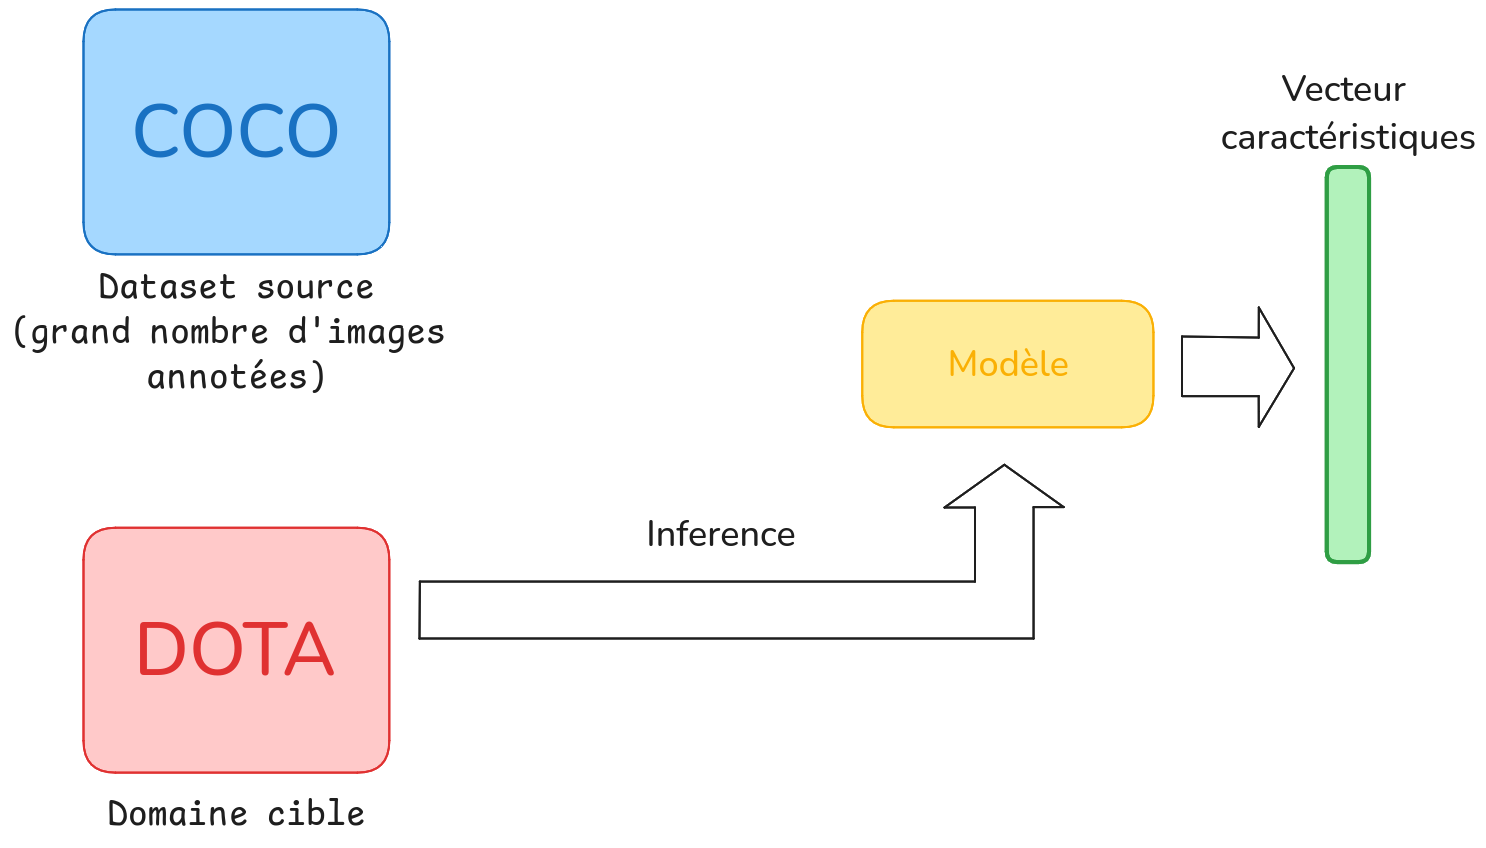
\includegraphics[width=\textwidth]{Figures/embeddings}
            \caption{Méthode utilisée pour extraire le vecteur des caractéristiques.
            L'idée est de remplacer la tête de classification par un module ROI pooling.}
        \end{figure}
    }
    \pause
    \only<3>{
        \begin{figure}
            \centering
            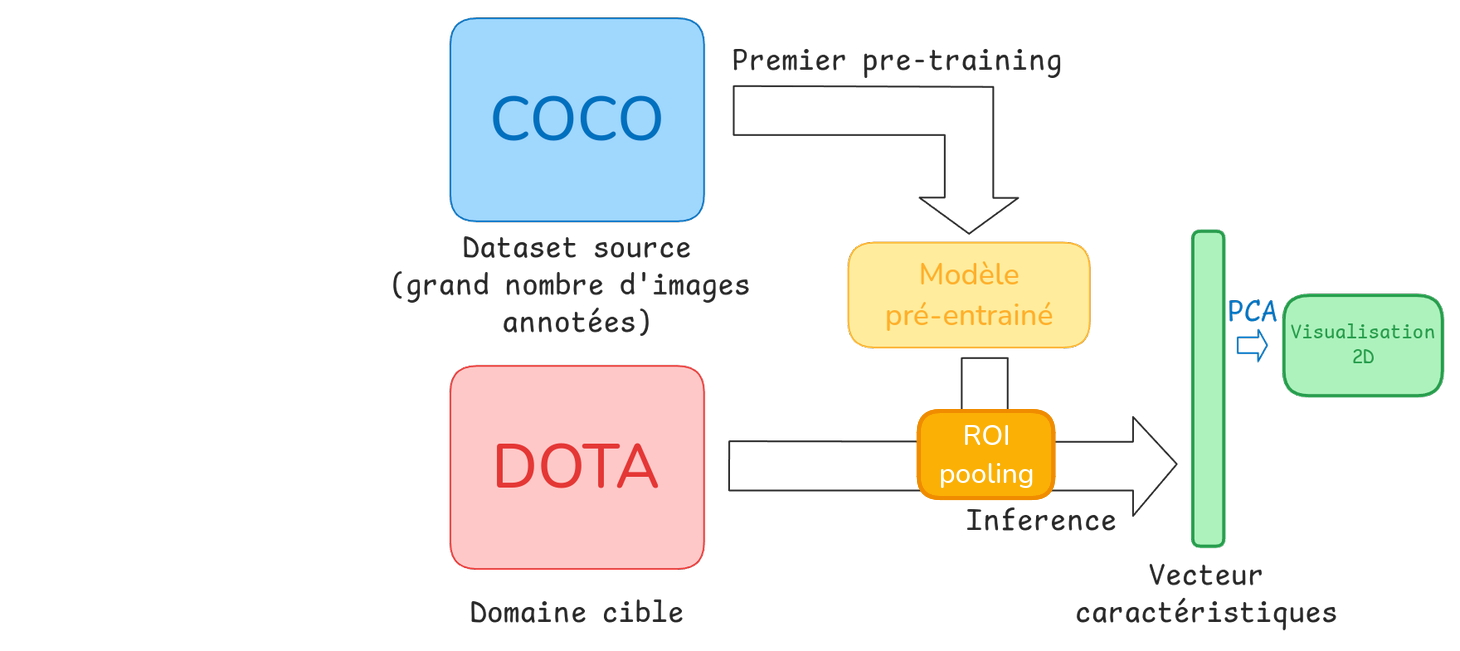
\includegraphics[width=\textwidth]{Figures/embeddings_pca}
            \caption{Méthode utilisée pour extraire le vecteur des caractéristiques.
            L'idée est de remplacer la tête de classification par un module ROI pooling.}
        \end{figure}
    }

\end{subsectionframemod}
    \begin{subsectionframemod}{Conclusion}
    \begin{figure}[!t]
        \centering
        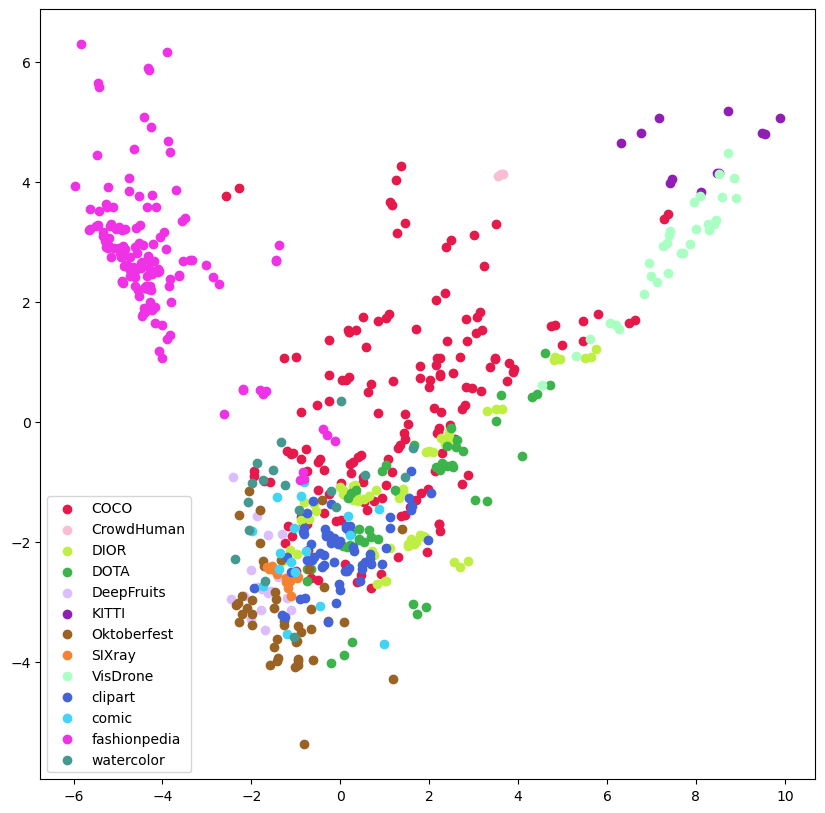
\includegraphics[width=0.6\textwidth]{Figures/2d_class_plot.png}
        \caption{Représentation 2D des projections des barycentres de chaque classe, obtenue après le passage des images de chaque dataset dans un modèle pré-entraîné sur COCO, suivi d'une réduction dimensionnelle par PCA.}
        \label{fig:2dclass}
    \end{figure}
\end{subsectionframemod}



    \begin{subsectionframemod}{Difference between Natural and Aerial Images}
    \begin{figure}[!h]
    \centering
    \begin{tabular}{cc}
        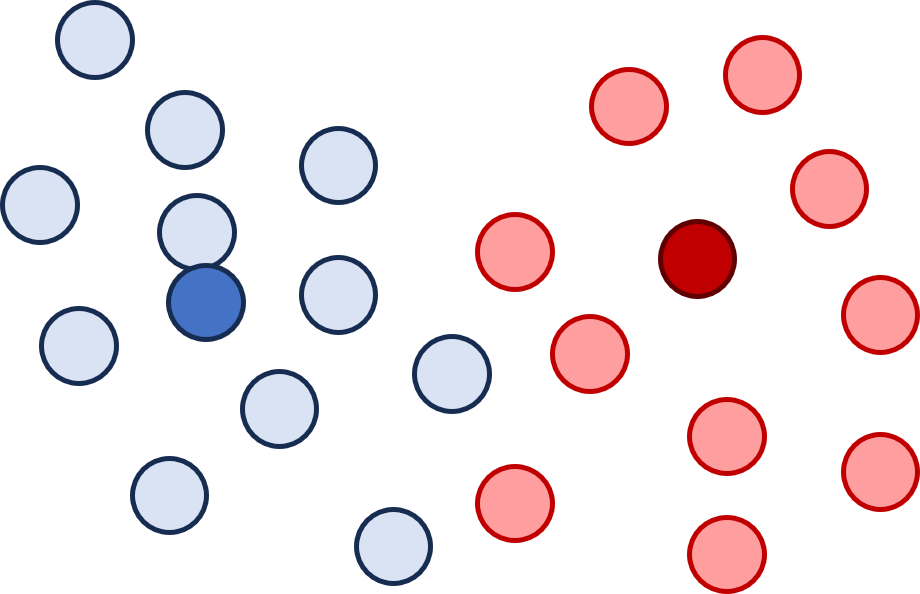
\includegraphics[scale=0.25]{Figures/con_sep.png} &
        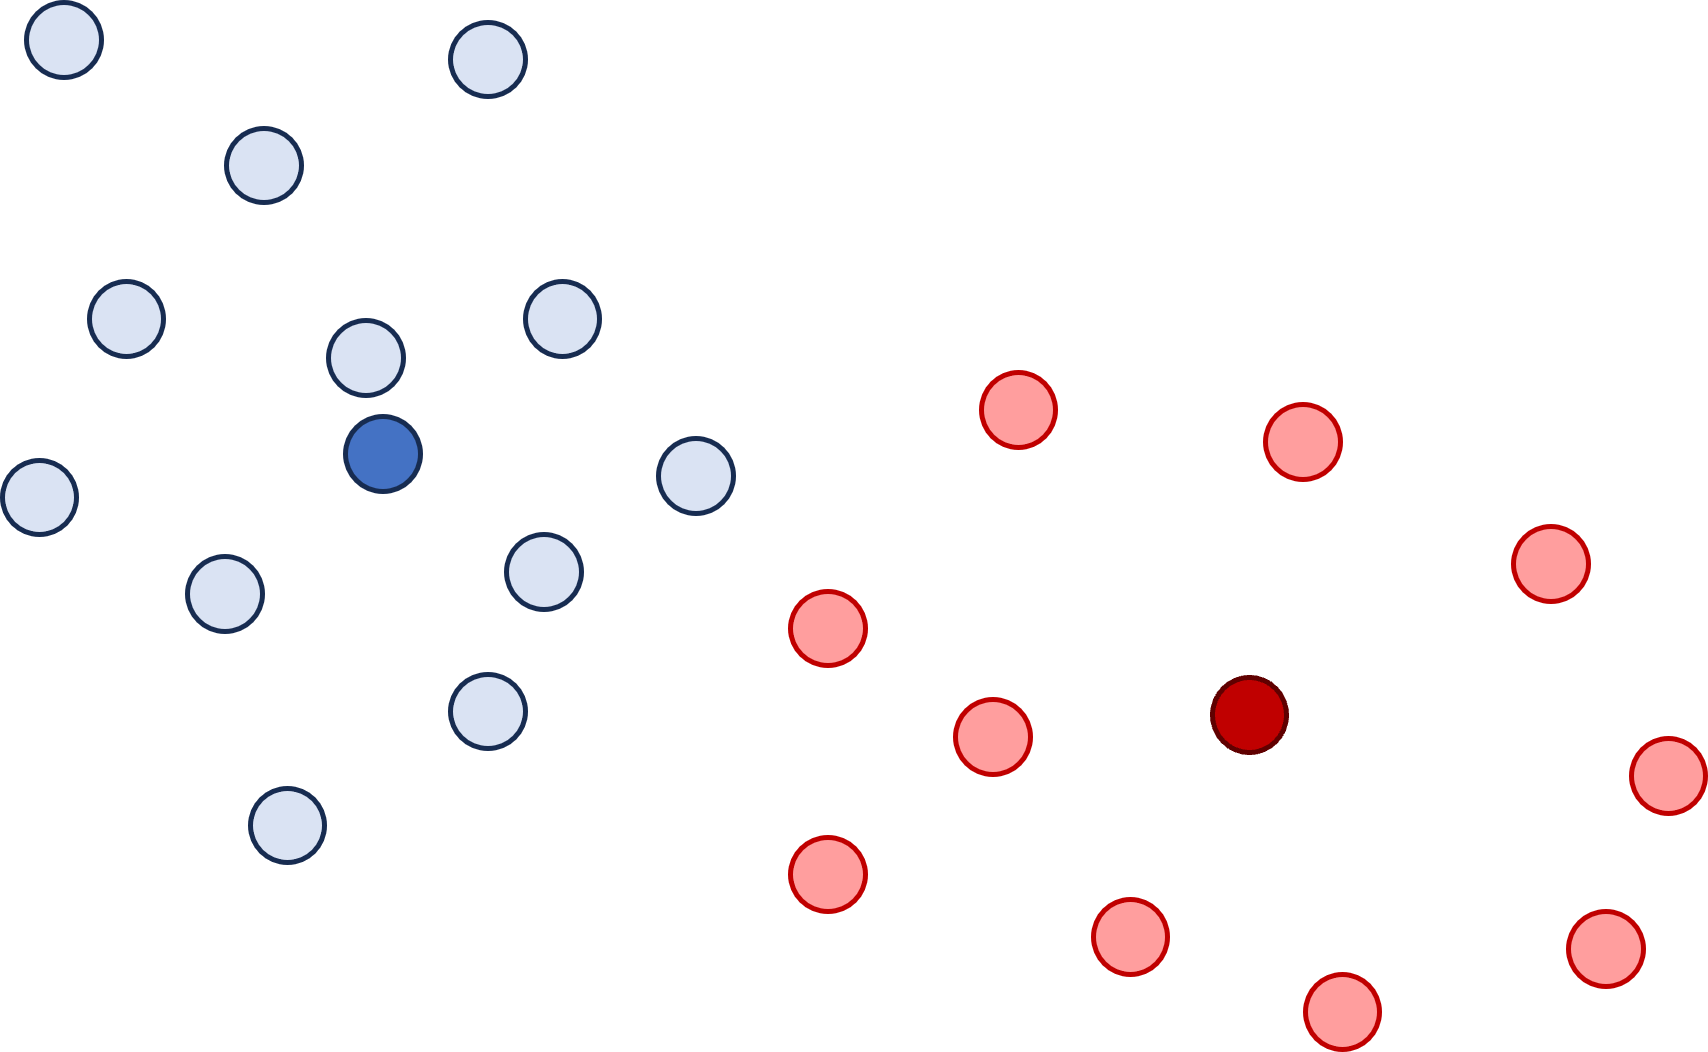
\includegraphics[scale=0.25]{Figures/ncon_sep.png} \\
        (a) Variance intra-classe faible, & (b) Variance intra-classe forte,\\
         Variance inter-classe forte, & Variance inter-classe forte, \\
         \\
        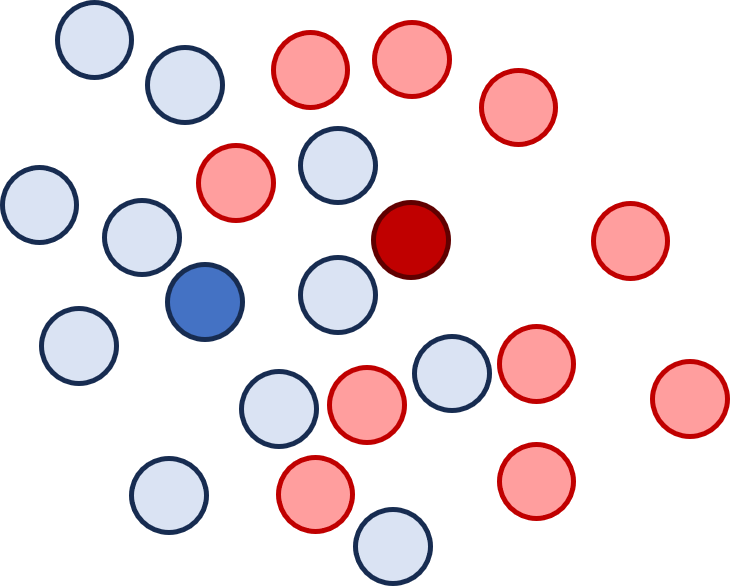
\includegraphics[scale=0.25]{Figures/con_nsep.png} &
        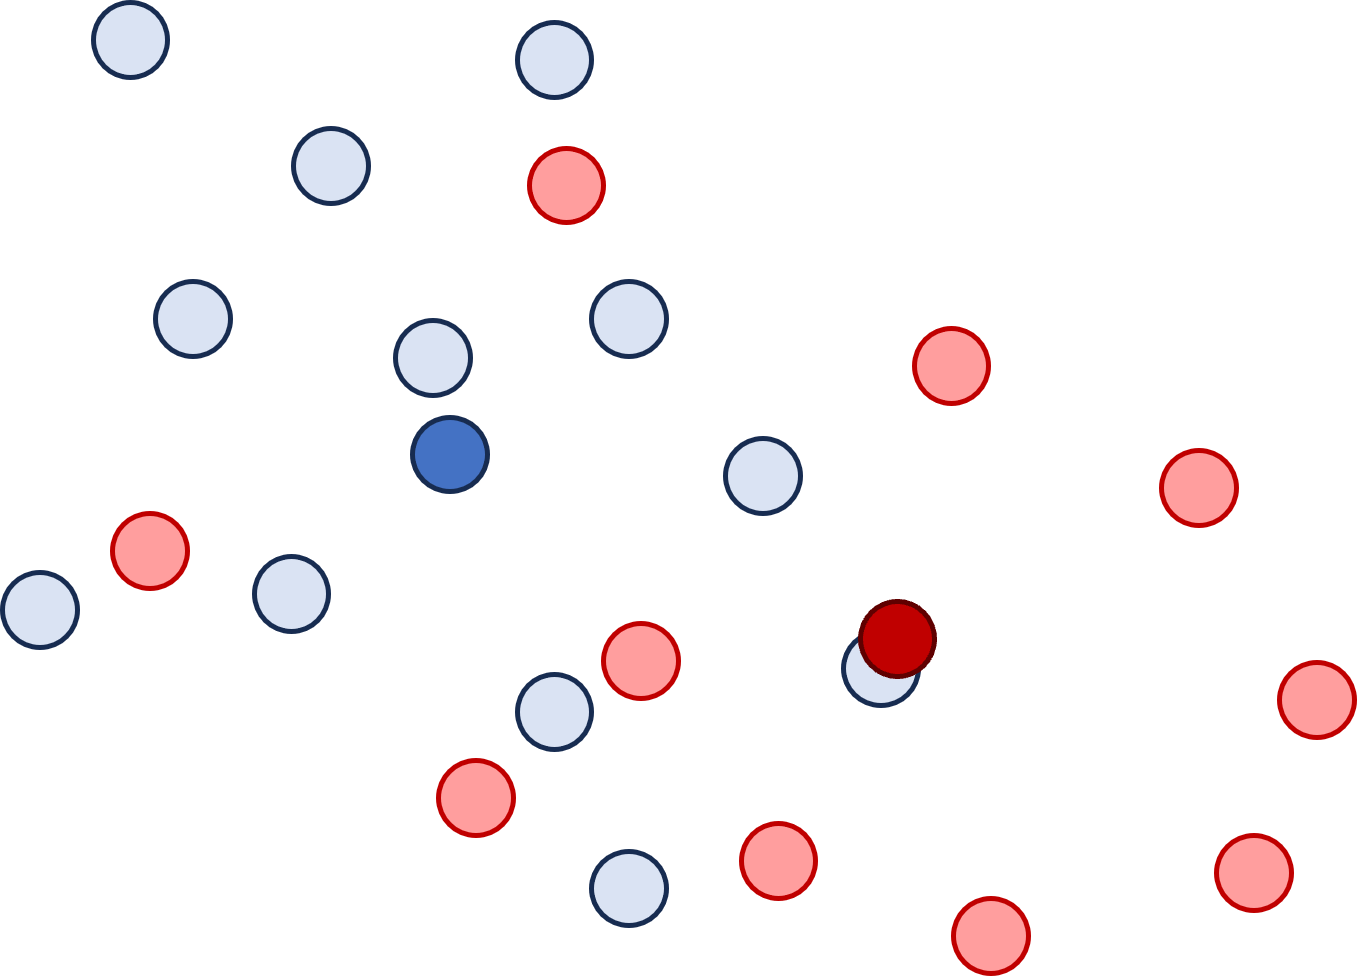
\includegraphics[scale=0.25]{Figures/ncon_nsep.png}\\
        (d) Variance intra-classe faible, & (c) Variance intra-classe forte, \\
        Variance inter-classe faible,  & Variance inter-classe faible, \\
    \end{tabular}
    \caption{Illustration conceptuelle de la séparabilité des classes en relation avec les variances inter-classes et intra-classes. Les projections dans l'espace latent des images d'une classe sont représentées par des points bleus, tandis que les projections d'une autre classe sont marquées en rouge, avec les barycentres de chaque classe indiqués par des points plus foncés.}
    \label{fig:sep_classes}
\end{figure}
\end{subsectionframemod}




    \begin{subsectionframemod}{Conclusion}
    \begin{figure}[!t]
        \centering
        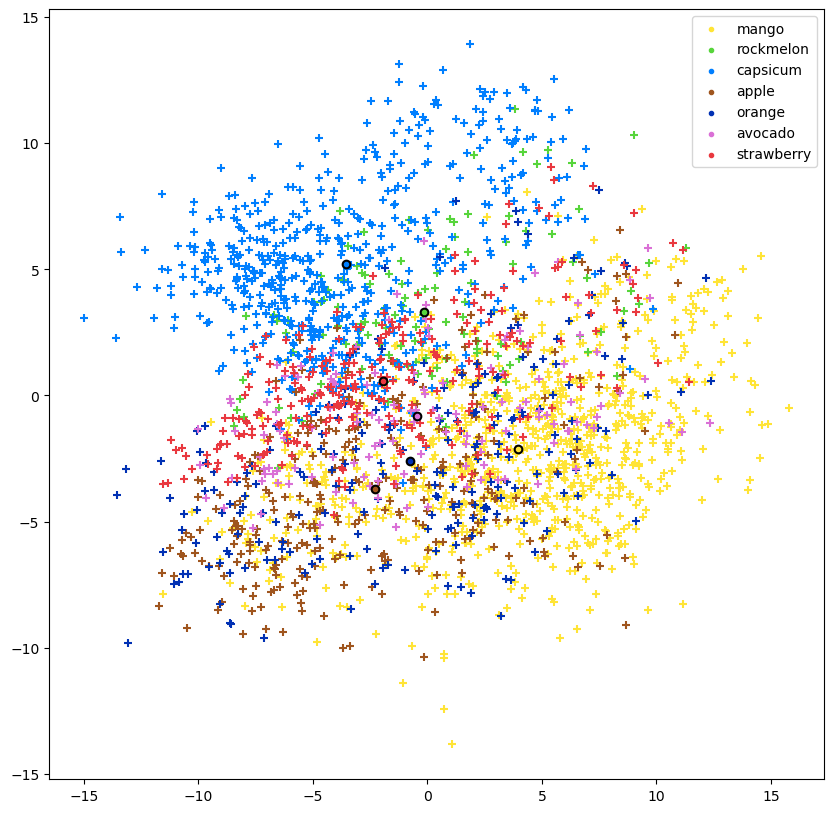
\includegraphics[width=0.6\textwidth]{Figures/deepfruits.png}
        \caption{Représentation 2D de la projection des objets de DeepFruits, obtenue après le passage des images de chaque dataset dans un modèle pré-entraîné sur COCO, suivi d'une réduction dimensionnelle par PCA. Les barycentres mis en valeur avec des cercles de couleurs.}
        \label{fig:deepfruits}
    \end{figure}
\end{subsectionframemod}




    \subsection{Méthodes PEFT (Parameter Efficient Fine-Tuning) pour limiter l'overfitting}\label{sec:peft}
    \begin{subsectionframemod}{Difference between Natural and Aerial Images}
    \metroset{block=fill}
    \begin{alertblock}{LoRA (Low-Rank Adaptation)}
        LoRA (Low-Rank Adaptation) est une technique d'optimisation qui ajuste efficacement les modèles de réseaux neuronaux de grande taille en réduisant le nombre de paramètres à ajuster via la factorisation des matrices de poids.
        En limitant le nombre de paramètres modifiés, elle aide également à réduire le risque d'overfitting tout en maintenant de bonnes performances.
    \end{alertblock}
    \vspace{5mm}

    \begin{figure}
        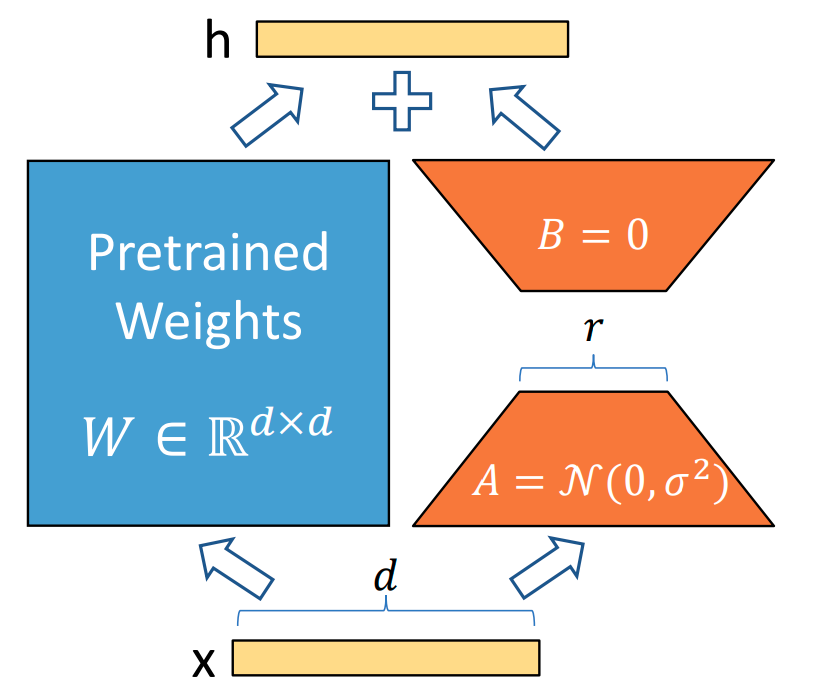
\includegraphics[width=0.4\textwidth]{Figures/lora.png}
        \caption{Principe de l'entrainement LoRA. Ici on entraine seulement A et B (\cite{lora}).}
    \end{figure}


\end{subsectionframemod}
    \begin{subsectionframemod}{Difference between Natural and Aerial Images}

    \begin{figure}
        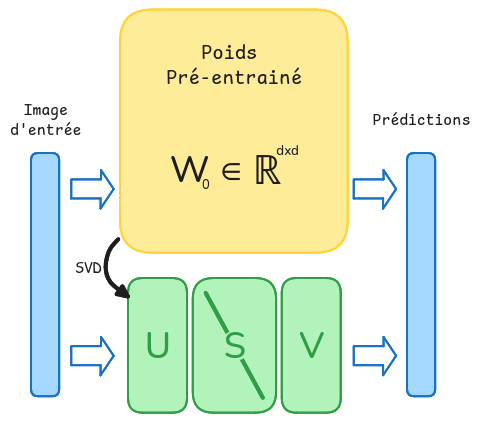
\includegraphics[width=0.4\textwidth]{Figures/svf.png}
        \caption{SVF (\cite{sun2022singular}) se base sur une décomposition en valeurs singulières. Dans ce cas, on entraîne seulement les valeurs singulières.}
    \end{figure}


\end{subsectionframemod}

    \subsection{Premiers résultats avec LoRA}\label{subsec:results-loracurves}
    \begin{subsectionframemod}{Performance Analysis}

\begin{figure}[h]
        \centering
        \begin{subfigure}{0.3\textwidth}
            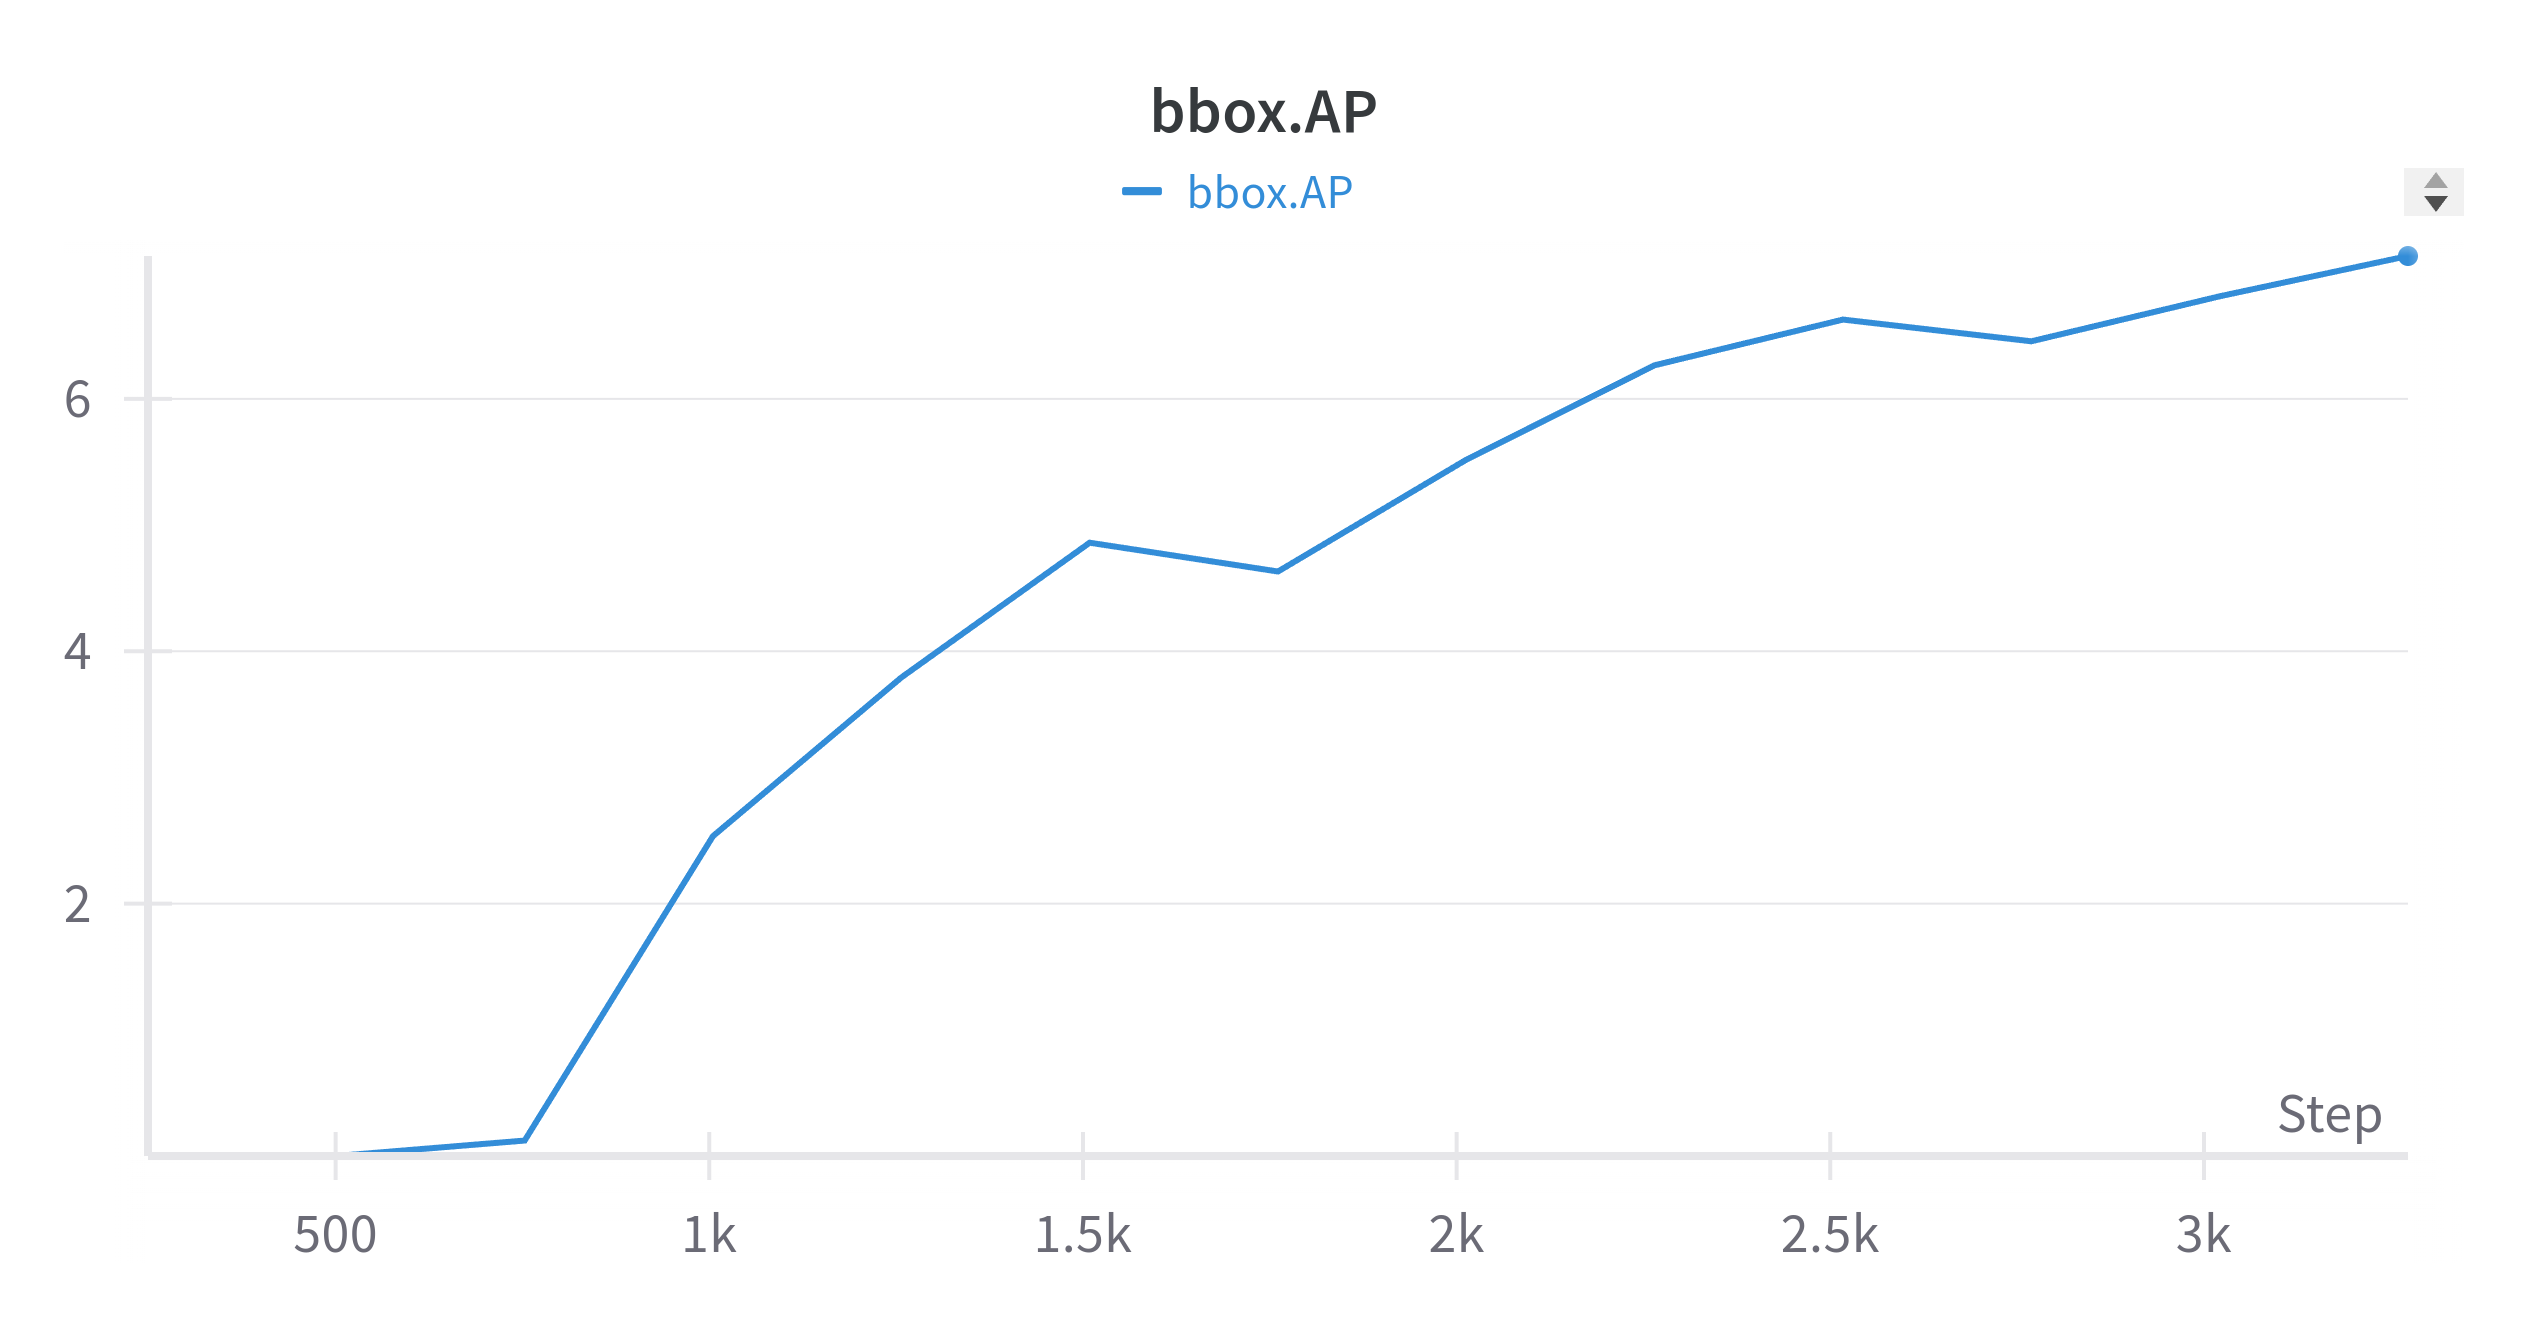
\includegraphics[width=\textwidth]{Figures/lora1.png}
        \end{subfigure}
        \begin{subfigure}{0.3\textwidth}
            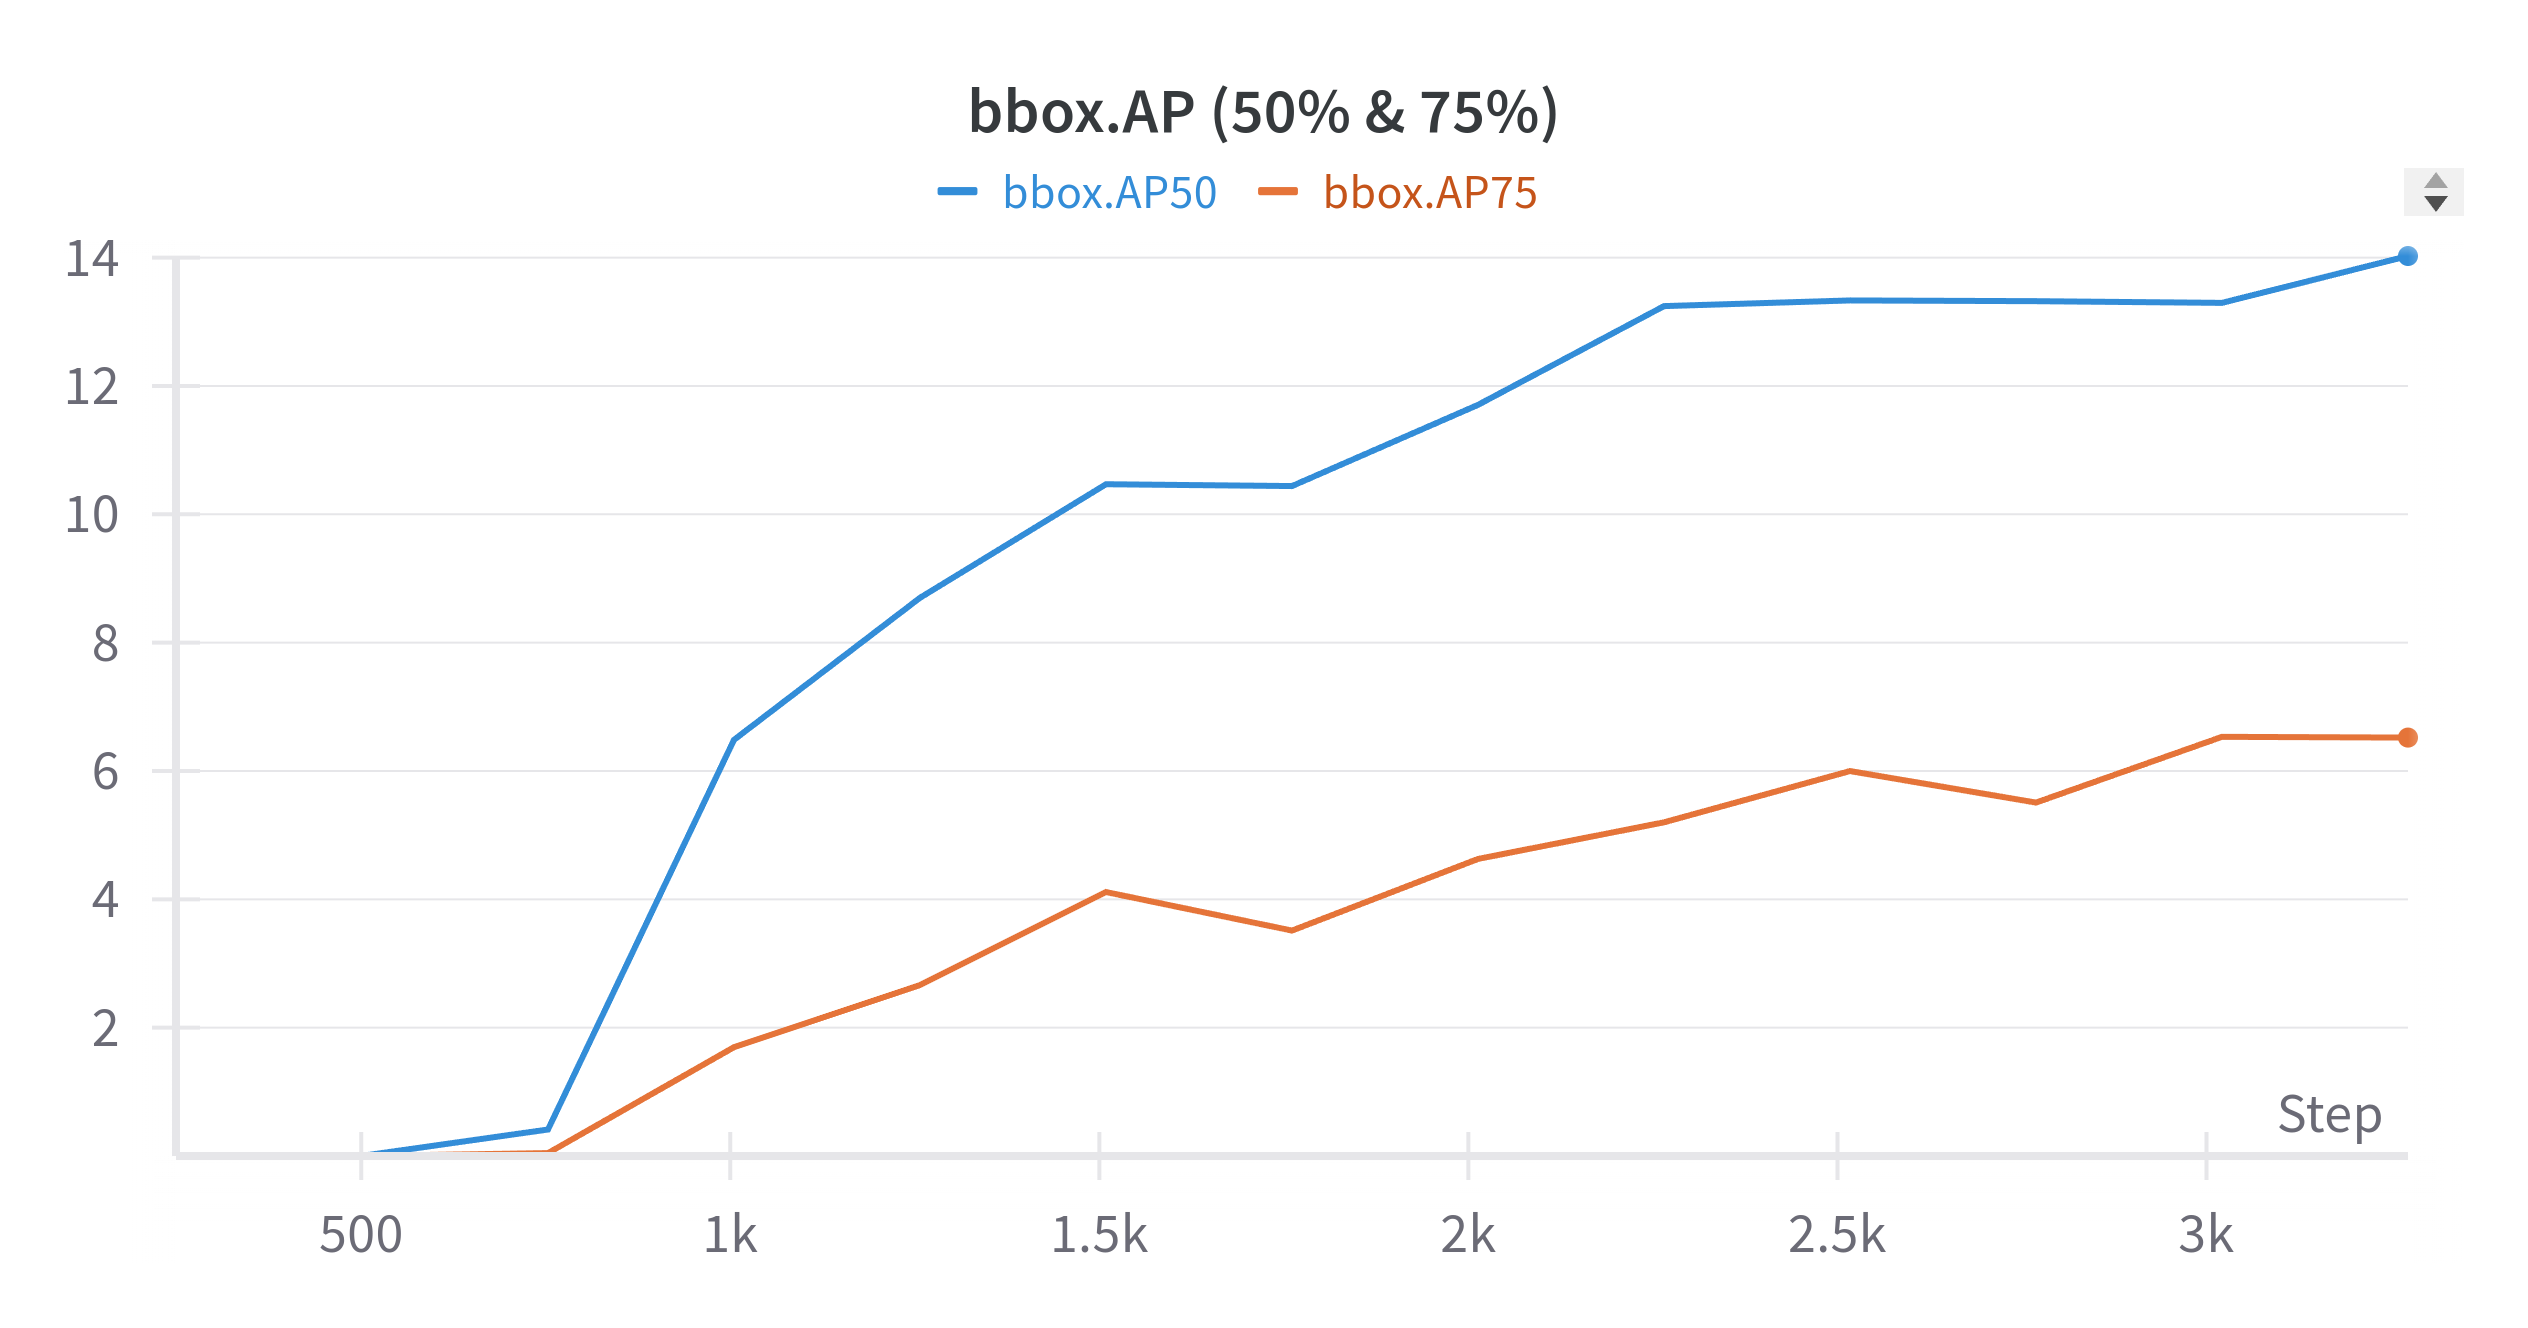
\includegraphics[width=\textwidth]{Figures/lora2.png}
        \end{subfigure}
        \begin{subfigure}{0.3\textwidth}
            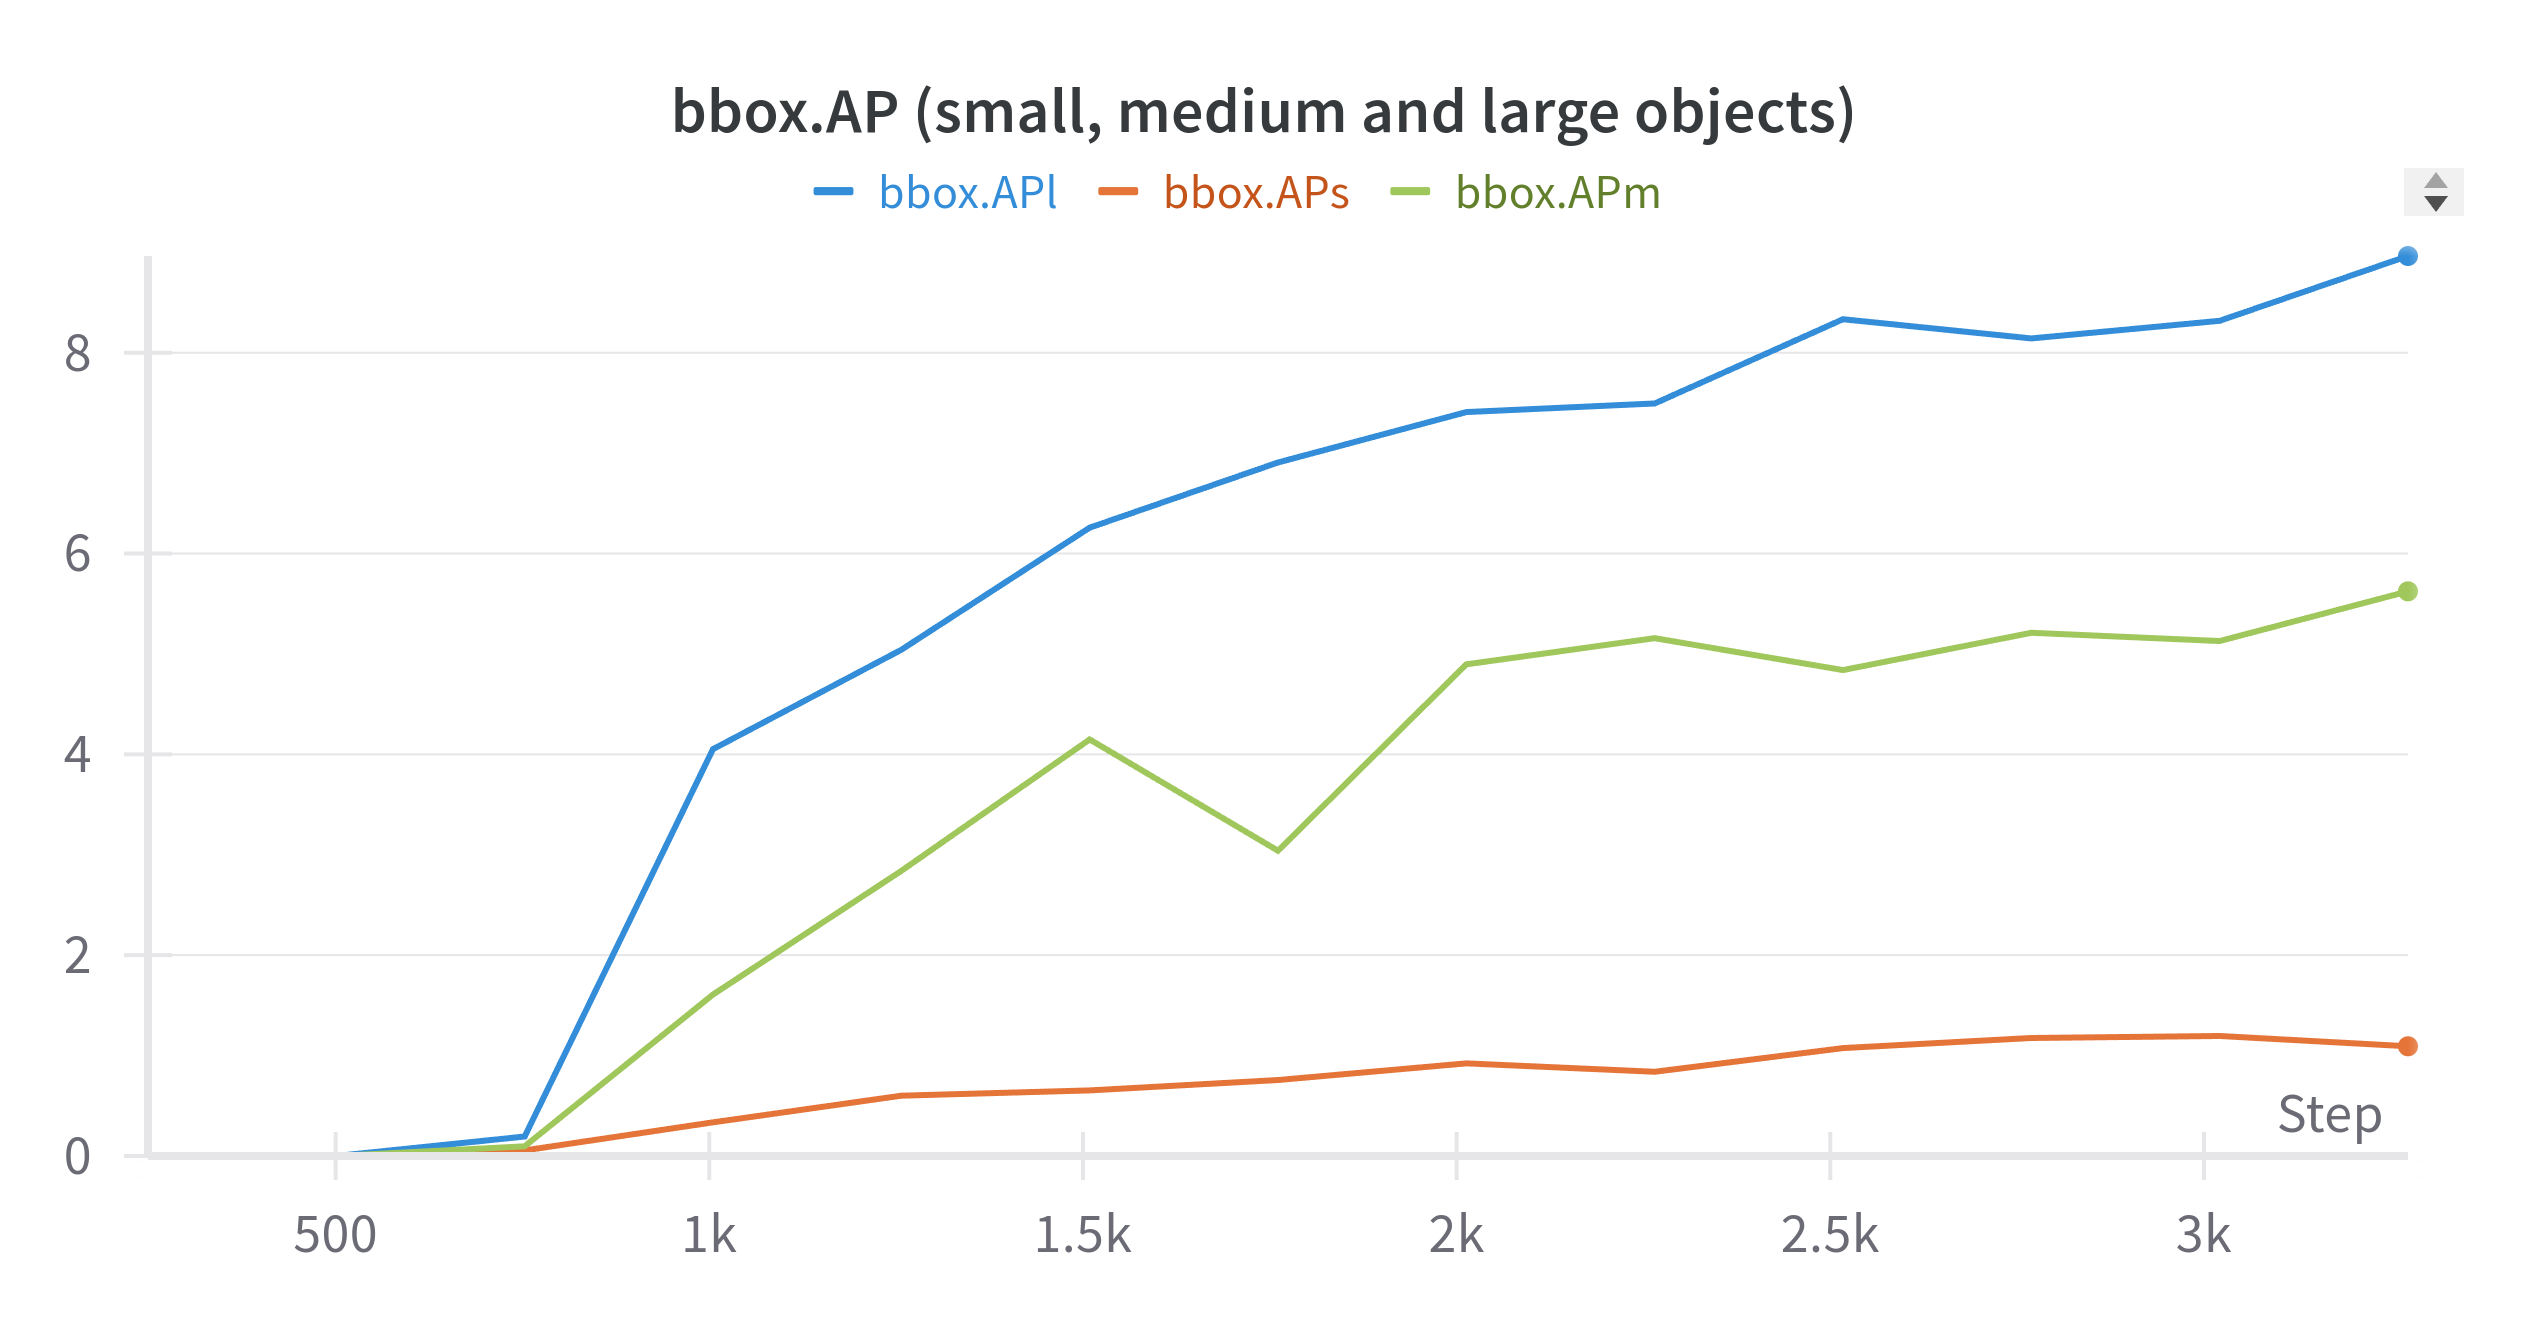
\includegraphics[width=\textwidth]{Figures/lora3.png}
        \end{subfigure}
        \begin{subfigure}{0.3\textwidth}
            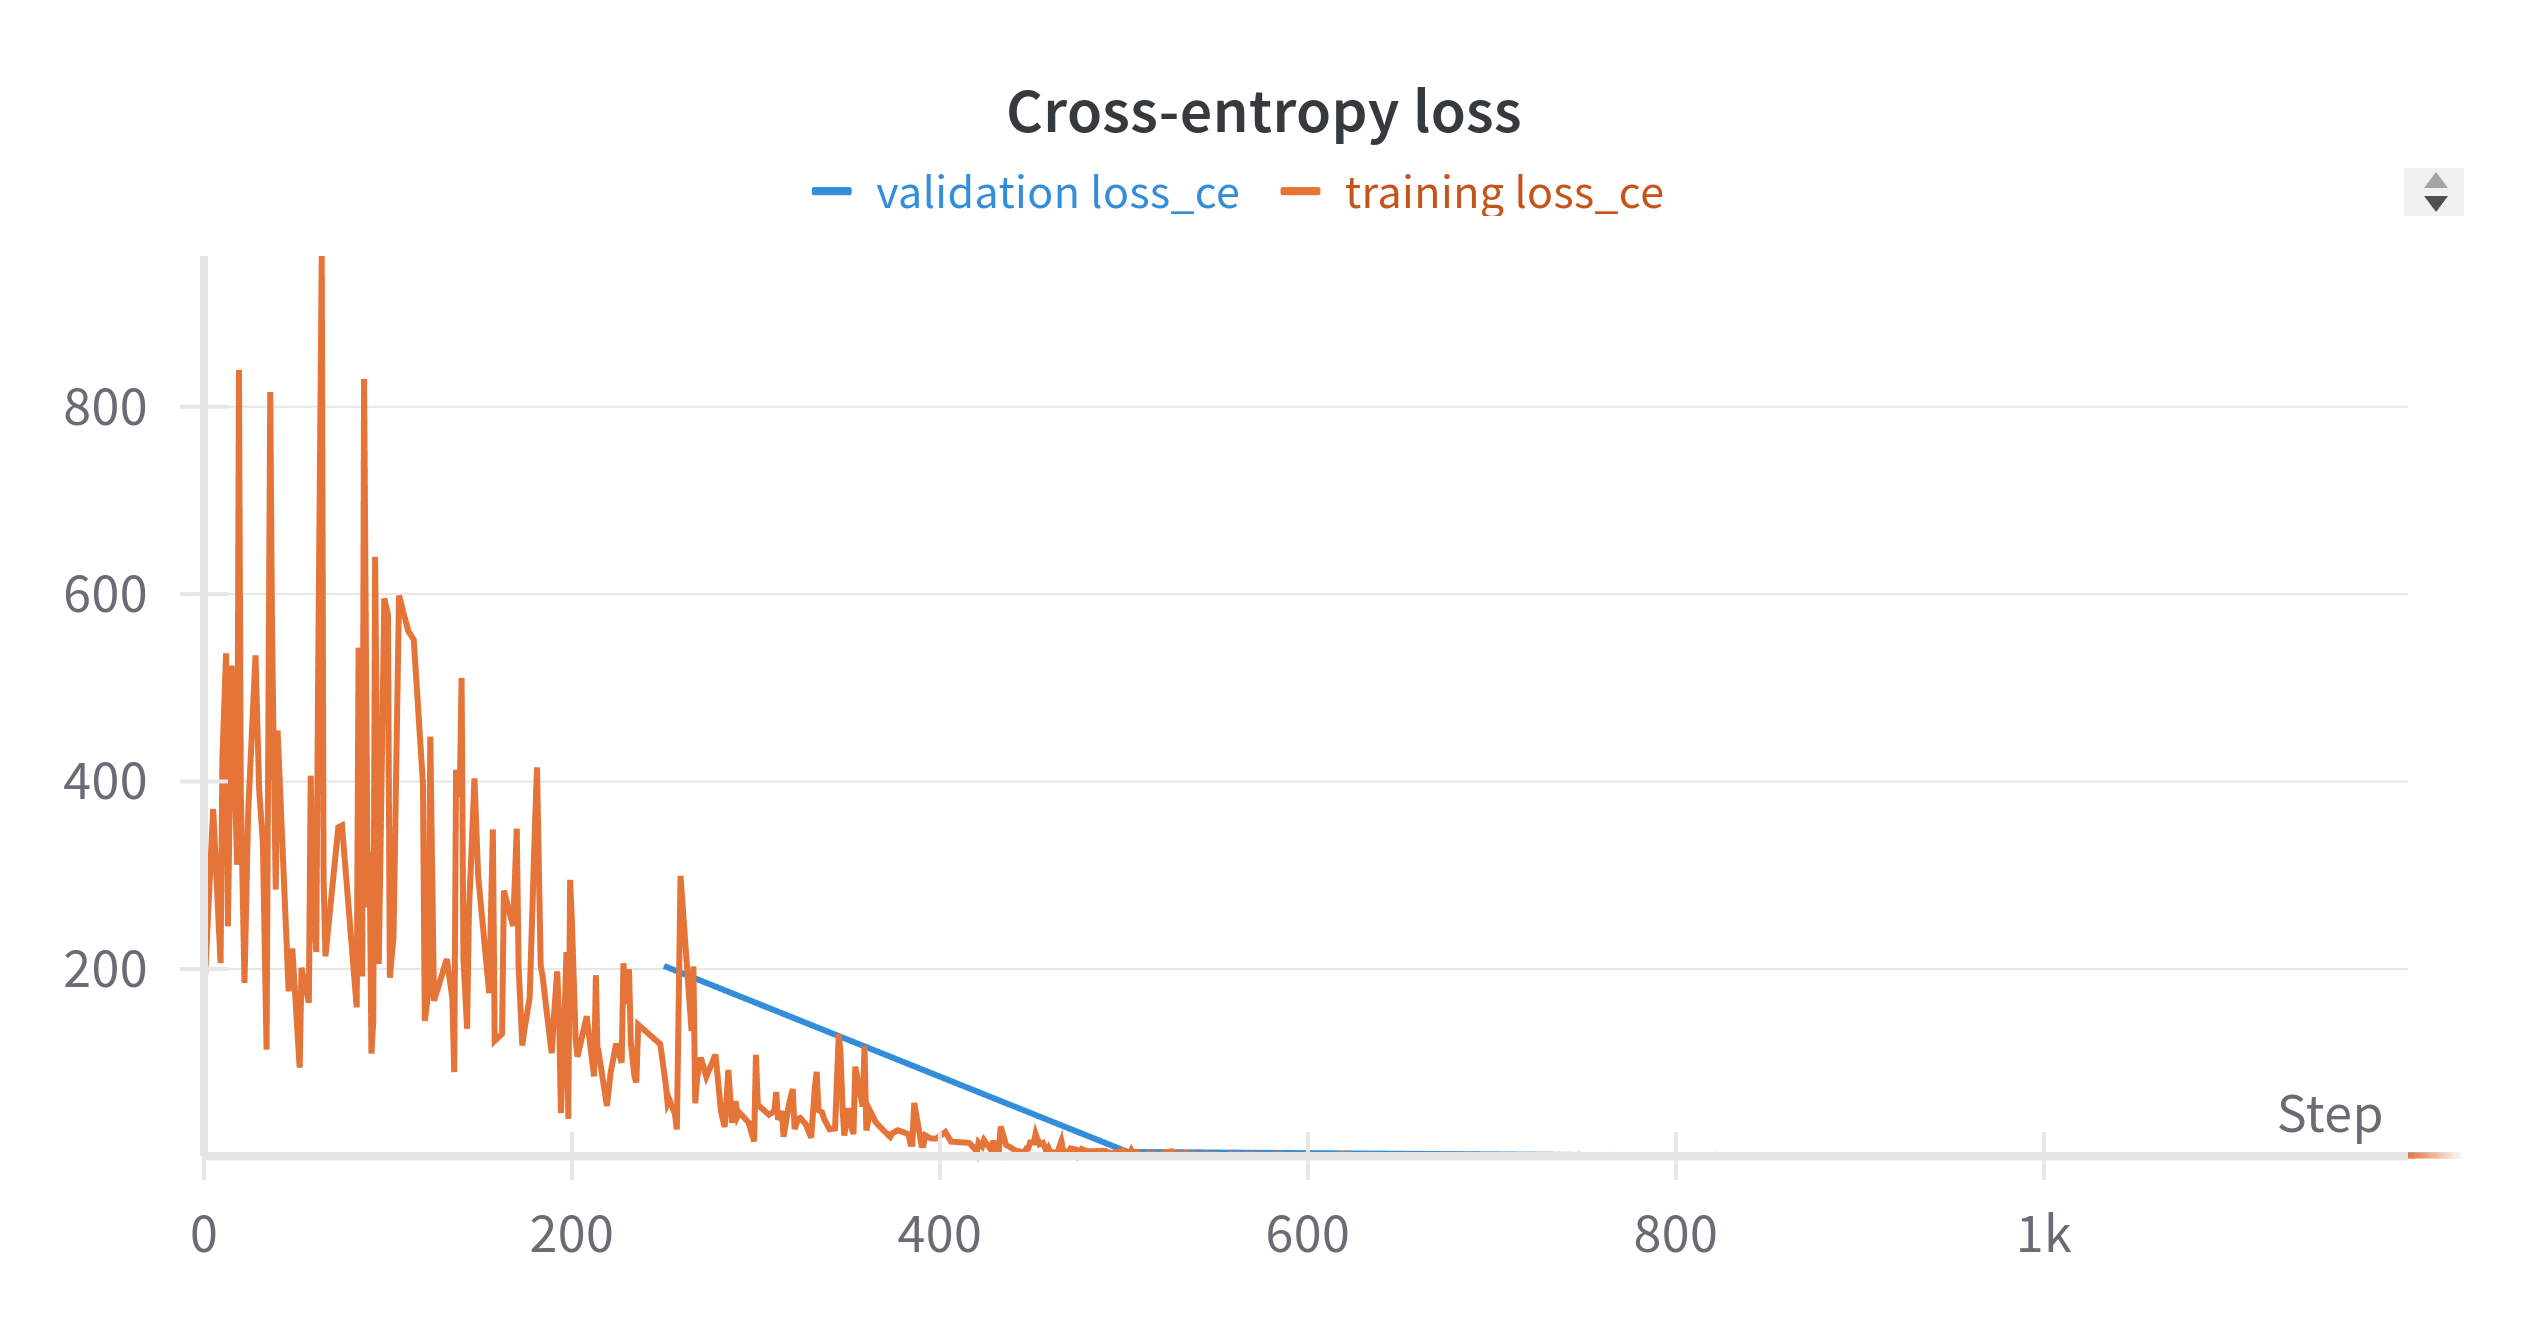
\includegraphics[width=\textwidth]{Figures/lora4.png}
        \end{subfigure}
        \begin{subfigure}{0.3\textwidth}
            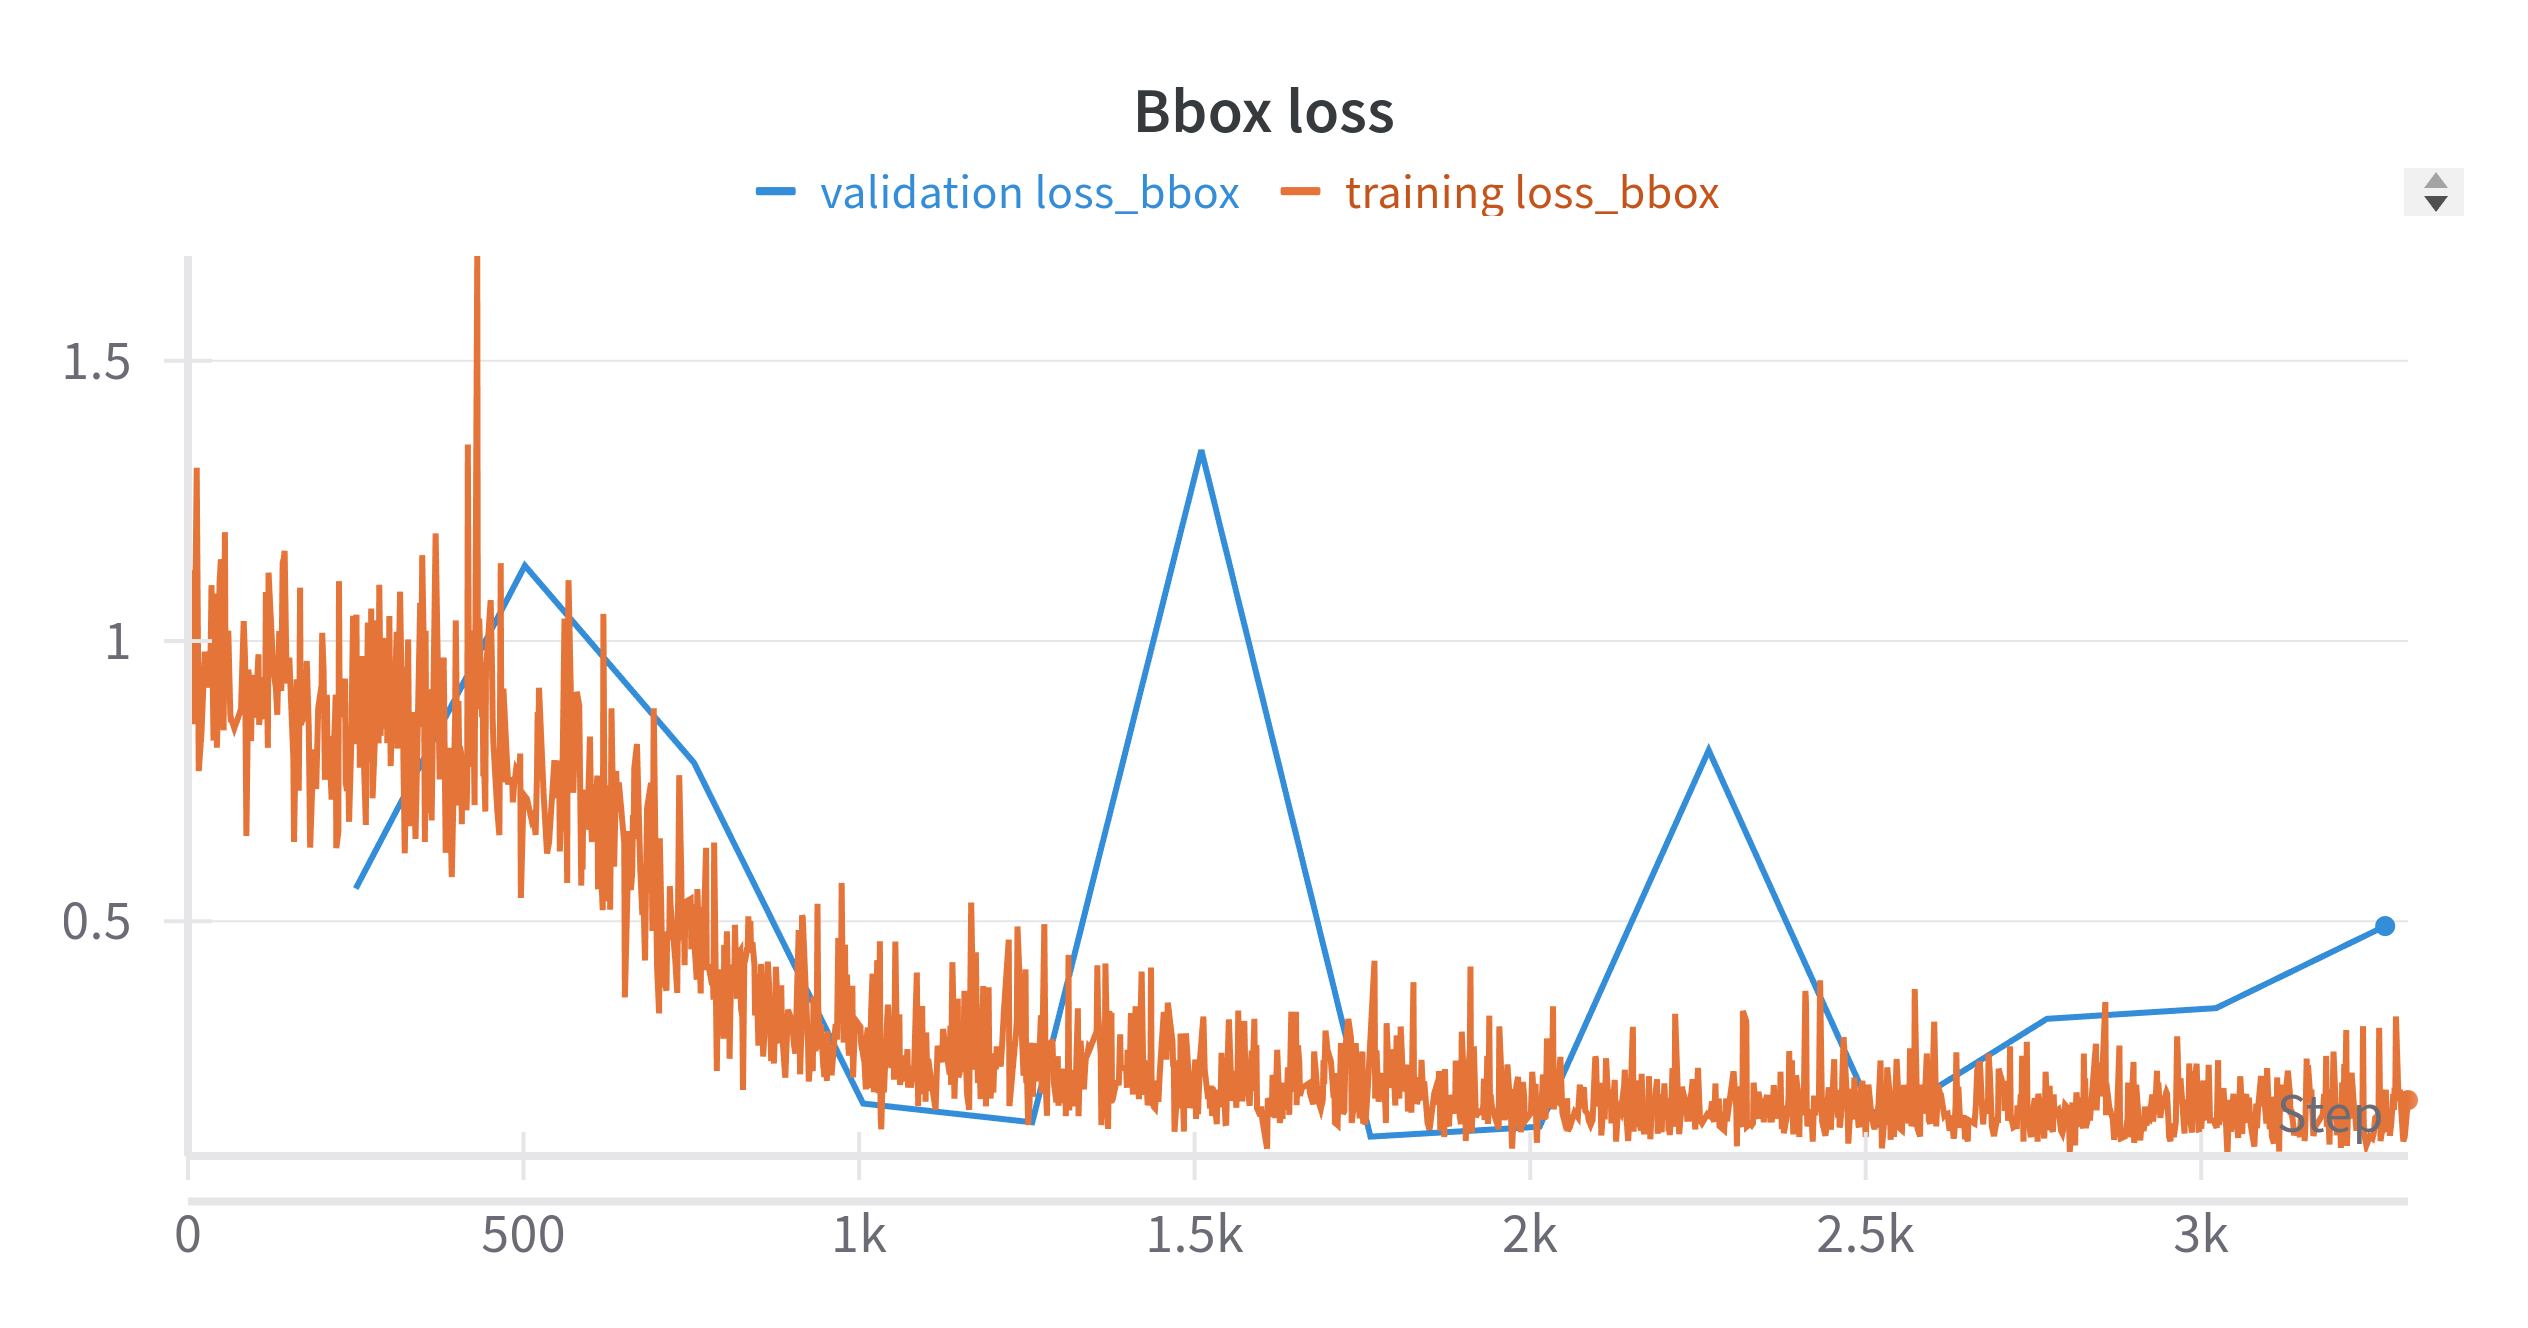
\includegraphics[width=\textwidth]{Figures/lora5.png}
        \end{subfigure}
        \caption{Impact de LoRA sur l'entraînement de FSDiffusionDet sur DIOR en utilisant 10 shots.}
        \label{fig:lora_curves}
    \end{figure}
\end{subsectionframemod}




    \section{Contributions scientifiques}\label{subsec:approach-publications}
    \begin{subsectionframemod}{Publications}
    \textbf{Articles de conférence acceptés (avant la thèse)} :
    \begin{itemize}
        \item[-] Straightforward Adaptation of Particle Filter to Fish Eye Images for Top View Pedestrian Tracking -- publié à \bfalert{ICASSP}
        (14 avr. 2024)
        \item[-] Improving Few-Shot and Cross-Domain Object Detection on Aerial Images with a Diffusion-Based Detector --
        accepté et présenté à \bfalert{IGARSS} (7 Juil. 2024) (relecture, participation aux expériences et présentation)
    \end{itemize}

    \textbf{Article de journal accepté (avant la thèse)} :
    \begin{itemize}
        \item[-] Human tracking in top-view fisheye images: Analysis of familiar similarity measures via HOG
        and against various color spaces  -- publié à \bfalert{Journal of Imaging}
        (16 avr. 2022).
    \end{itemize}

    \textbf{Articles de conférence soumis}
    \begin{itemize}
        \item[-] Indirect Attention: IA-DETR for one shot Object Detection -- soumis à \bfalert{ICLR} (2024) (participation au code et aux expériences)
    \end{itemize}

\end{subsectionframemod}



    \section{Formations}\label{subsec:formations}
    \begin{subsectionframemod}{Publications}
    \textbf{Formation dotorale suivie} :
    \begin{itemize}
        \item[-] Formations professionnalisantes et langues -- Anglais de communication niveau faux débutant-intermédiaire  \bfalert{4 ECTS}
    \end{itemize}

    \textbf{Conférences présentées} :
    \begin{itemize}
        \item[-] Présentation orale à \bfalert{IGARSS} (8-12 Juil.) -- \textit{Improving Few-Shot and Cross-Domain Object Detection on Aerial Images with a Diffusion-Based Detector} \bfalert{24 ECTS}
    \end{itemize}

    \textbf{Mobilité} :
    \begin{itemize}
        \item[-] Mobilité de 4 mois à l'ETS Montréal (Canada)
    \end{itemize}

\end{subsectionframemod}



    \section{Travaux futurs}\label{subsec:approach-future-work}
    \begin{subsectionframemod}{Conclusion}
\begin{itemize}
    \item[-]  Rédaction d'un article benchmark sur les méthodes cross-domain few-shot incluant les différents fine-tuning et les estimations du domain shift.
    \item[-]  Étude des PEFT pour la regression.
    \item[-]  Étudier l'apport des les VLM (Vision/Language Models) sur le cross-domain few-shot.
    \item[-]  Compléter le gros des formations doctorales internes obligatoires et non obligatoires.
\end{itemize}


\end{subsectionframemod}


    \usebeamertemplate{endpage}

    \begin{frame}[allowframebreaks=]{References}
        \printbibliography
    \end{frame}
\end{document}
